\chapter{Viability of neuronal cultures in microfluidic devices in static conditions and under steady flow}
\label{chap:devicesAndFlow}


\section{Introduction}
\label{sec:devices:introduction}
As outlined in section \ref{sec:introduction:objs} the purpose of this Ph.D work is to produce a model for phasic neuromodulator signalling by generating rapid agonist transients onto an entire neuronal culture. This is to be achieved using the interface shifting method in microfluidic devices (see section \ref{sec:introduction:mufdDrugDelivery}). As we will show, successfully applying this method to generate transients at time scales mimicking phasic neuromodulator signalling involves rapid flow rates in the order of \(1 mm\cdot s^{1}\). Previous microfluidics work involving primary neurons used such rapid flow rates but just for short experiments lasting between minutes to 2 hours at most \cite{biffi2012microfluidic,morel2012amplification,wang2008microfluidics,pearce2005integrated}. Studies showing long term neuronal culture development under flow used much reduced flow rates where the convective forces were comparable to diffusion \cite{choi2013neurotoxic,millet2007microfluidic,park2015three,kumamoto2015effects}. Thus to avoid the complexity involved in getting neuronal cultures to survive long term under rapid flow we elected to follow an experimental paradigm whereby the cultures were initially grown in microfluidic devices in static conditions. After reaching maturity they were subjected to flow only for the duration of the experimental session. The first part of this chapter is dedicated to development of a protocol for long term culturing of primary rat neurons in microfluidic devices. As reviewed in section \ref{sec:introduction:mufdNeuroscience}, this type of protocol is prevalent in the literature but the configuration of our devices, which were designed with the interface shifting method in mind, required specific adaptations.

An important part of the our experimental design is for the culture to be of restricted size (i.e., a microculture). This is necessary, firstly, because the interface shifting routine involves having a small proportion of the microfluidic channel area chronically exposed to the agonist, even between transients (see section \ref{sec:introduction:mufdDrugDelivery}). Thus to avoid such chronic drug exposure, the culture needs to be located entirely outside the chronically exposed area. Secondly, it is important to note that an agonist pulse in the interface shifting method actually takes the form of an agonist wave travelling along the long axis of the channel. This means that, depending on the flow rate and the geometry of the culture, cells at different locations along the channel may experience the drug at different times following the pulse command. In phasic neuromodulator signalling, the agonist molecules are secreted from nerve terminals that innervate the entire volume of the target tissue. Consequently, a neuromodulator pulse involves an approximately synchronous increase of agonist concentration over the entire innervated tissue followed by a decrease in concentration as the agonist molecules get locally re-uptaken \cite{arbuthnott2007space}. It is important to note that, due to inhomogeneities in the spatial distribution of the innervating neuromodulatory fibers, different parts of the tissue still exhibit some delays in exposure to the agonist depending on their proximity to neuromodulatory synapse clusters. Nevertheless, these delays are small compared to the time scales of the global pulse \cite{arbuthnott2007space,venton2003real}. Because of the functional importance of timing in the neuromodulator signalling, it is essential that the microfluidic model does not exhibit increased delays in arrival of the agonist to different parts of the culture as compared to the \textit{in vivo} tissue. To achieve the right timings, the flow speed and culture size need to be selected so that the drug traversal time across the culture matches the delays in the modeled tissue. Thus, the ability to control the culture size is crucial and the second part of this chapter will describe a method for generating microcultures which harbour small specific areas of the channel by utilizing microwells. The viability of these microcultures will be analyzed to establish their usability.

A final important topic that will be covered in this chapter is that of neuronal viability under rapid flow. Primary neurons are considered to be highly sensitive to shear stresses. Since this system is developed with long term plasticity in mind it is important to make sure that the culture is kept viable and functional for at least several hours under the applied shear stresses. It is also important to take into account that a functional neuronal tissue employs a large number of intrinsic volume transmission processes which comprise controlled secretion and uptake of active substances into the ECM (reviewed in section \ref{sec:introduction:volTrans}). These substances include neurotransmitters, hormones, neurotrophic and growth factors and are generally termed conditioning factors. Rapid flow is likely to interrupt these processes by changing the concentrations of the conditioning factors or their spatial distributions. Since microfluidic flow has been scarcely used with primary neuronal cultures the flow rate limits have not been established and it is currently unclear what is the impact of each of the above-mentioned factors, shear stress and conditioning removal, on the culture viability. To characterize the effect of these factors we performed a viability assay under flow with a range of flow rates and media conditioning levels.

\section{Long term neuronal cultures in microfluidic devices}
    \subsection{Development of protocol}
    \label{sec:devices:protocolDev}

    This section outlines the development of a protocol for long term culturing of primary hippocampal neurons in microfluidic devices. Long term culturing of cortical and hippocampal neurons has been established for over 30 years \cite{brewer1993optimized,romijn1984towards,ray1993proliferation}. Recently, there has been an emerging use of microfluidic devices to culture neurons with increased control over the topology and to access specific neuronal compartments \cite{park2006microfluidic,park2013advances,gross2007applications}. Nevertheless, neuronal cultures are infamous for their sensitivity to subtleties in the preparation technique and the materials that come in contact with the media or the cells and often require specific adaptations for the specific lab / application \cite{kaech2006culturing,millet2007microfluidic}. We first established the required device geometries for our application and the conditions required for long term neuronal culturing in them.

    Figure \ref{fig:devices:basicDimensions} shows the dimensions of the devices used in this study. The dimensions were selected so that, given the volumetric flow rates allowed by our flow system, a flow speed would be produced that is compatible with the desired agonist exposure times. Thus the main channel width was \(1.5 mm\) and the height was \(65 \mu m\) giving a cross section of \(\approx 0.1 \mu m^{2}\). Using a flow rate of \(100 nl/s\) gives an averaged flow speed of \(1 mm/s\). Assuming that the long dimension of the culture would be less than a millimeter and that the culture would be positioned less than a millimeter from the agonist port then the agonist should reach the culture within a second and clear it a second later, which is the correct order of magnitude for neuromodulator phasic signalling \cite{venton2003real}. These initial calculations indicate the required channel geometries. Detailed testing of solution exchange under flow are reported in chapter \ref{chap:microculturePulses}.

    The devices were bonded to glass cover slips using plasma bonding (see section \ref{sec:methods:bonding} for details and more illustration of the assembled devices), oven sterilized, and then subjected to PLL surface treatment as detailed in section \ref{sec:methods:surface}.

    Due to the need to interface with a flow system, the microfluidic devices used in this work were made with biopsy punched ports of \(\approx 0.8 mm\) diameter which allow connection to the flow tubing by simple pressure fitting. This design contrasts with standard neuroscience oriented microfluidic devices where the ports are typically of \(8 mm\) diameter (e.g., \cite{park2006microfluidic,robertson2014chemically,millet2007microfluidic}). In these standard devices the seeding proceeds through pipetting of the cell solution into the ports and allowing the cells to flow through the channel (flow is enabled by controlling for a differential media height across the inlet and outlet ports). In the case of these standard devices, the ports function as de facto reservoirs by holding a significant volume of media (\(400 \mu L\) each) and therefore protect the device from dehydration and serve as a source of nutrients. Due to the smaller port size in our devices, plating was performed by injecting the cells into the inlet port using a gel loading tip. The volume of injection was selected to be larger than the internal volume of the device so as to fully flood it with cells. The devices used here had an internal volume smaller than \(1 \mu L\) (figure \ref{fig:devices:basicDimensions}) and the injection volume was \(2 \mu L\). After completion of the injection the cells were left suspended in the channel volume and were allowed to settle down in the incubator. The lack of flow following the cell injection made this protocol more consistent than the flow based seeding in standard devices. In those cases too strong of a flow ends up in having most of the cells flow through the device without settling and therefore in inconsistent seeding densities. On the other hand, a down side to our design is that due to their smaller diameter, the ports in our devices only hold about \(2.5 \mu L\) of media each and therefore cannot effectively fulfill the role of media reservoirs.

    The following subsections will outline the major steps taken during the development of the protocol to circumvent the issues encountered along the way. The development of the protocol was an iterative process, where pragmatic progress was prioritised over statistical testing of each step. The goal was to identify a strategy for reliably seeding channels with viable neurons that was reproducible and met the design criteria needed for rapid delivery of neuromodulators. Accordingly, a detailed analysis of the factors determining neuronal viability was not carried out but is presented in the form of examples and heuristics for the benefit of scientists wishing to use these techniques.

      \begin{figure}[h]
           \centering
            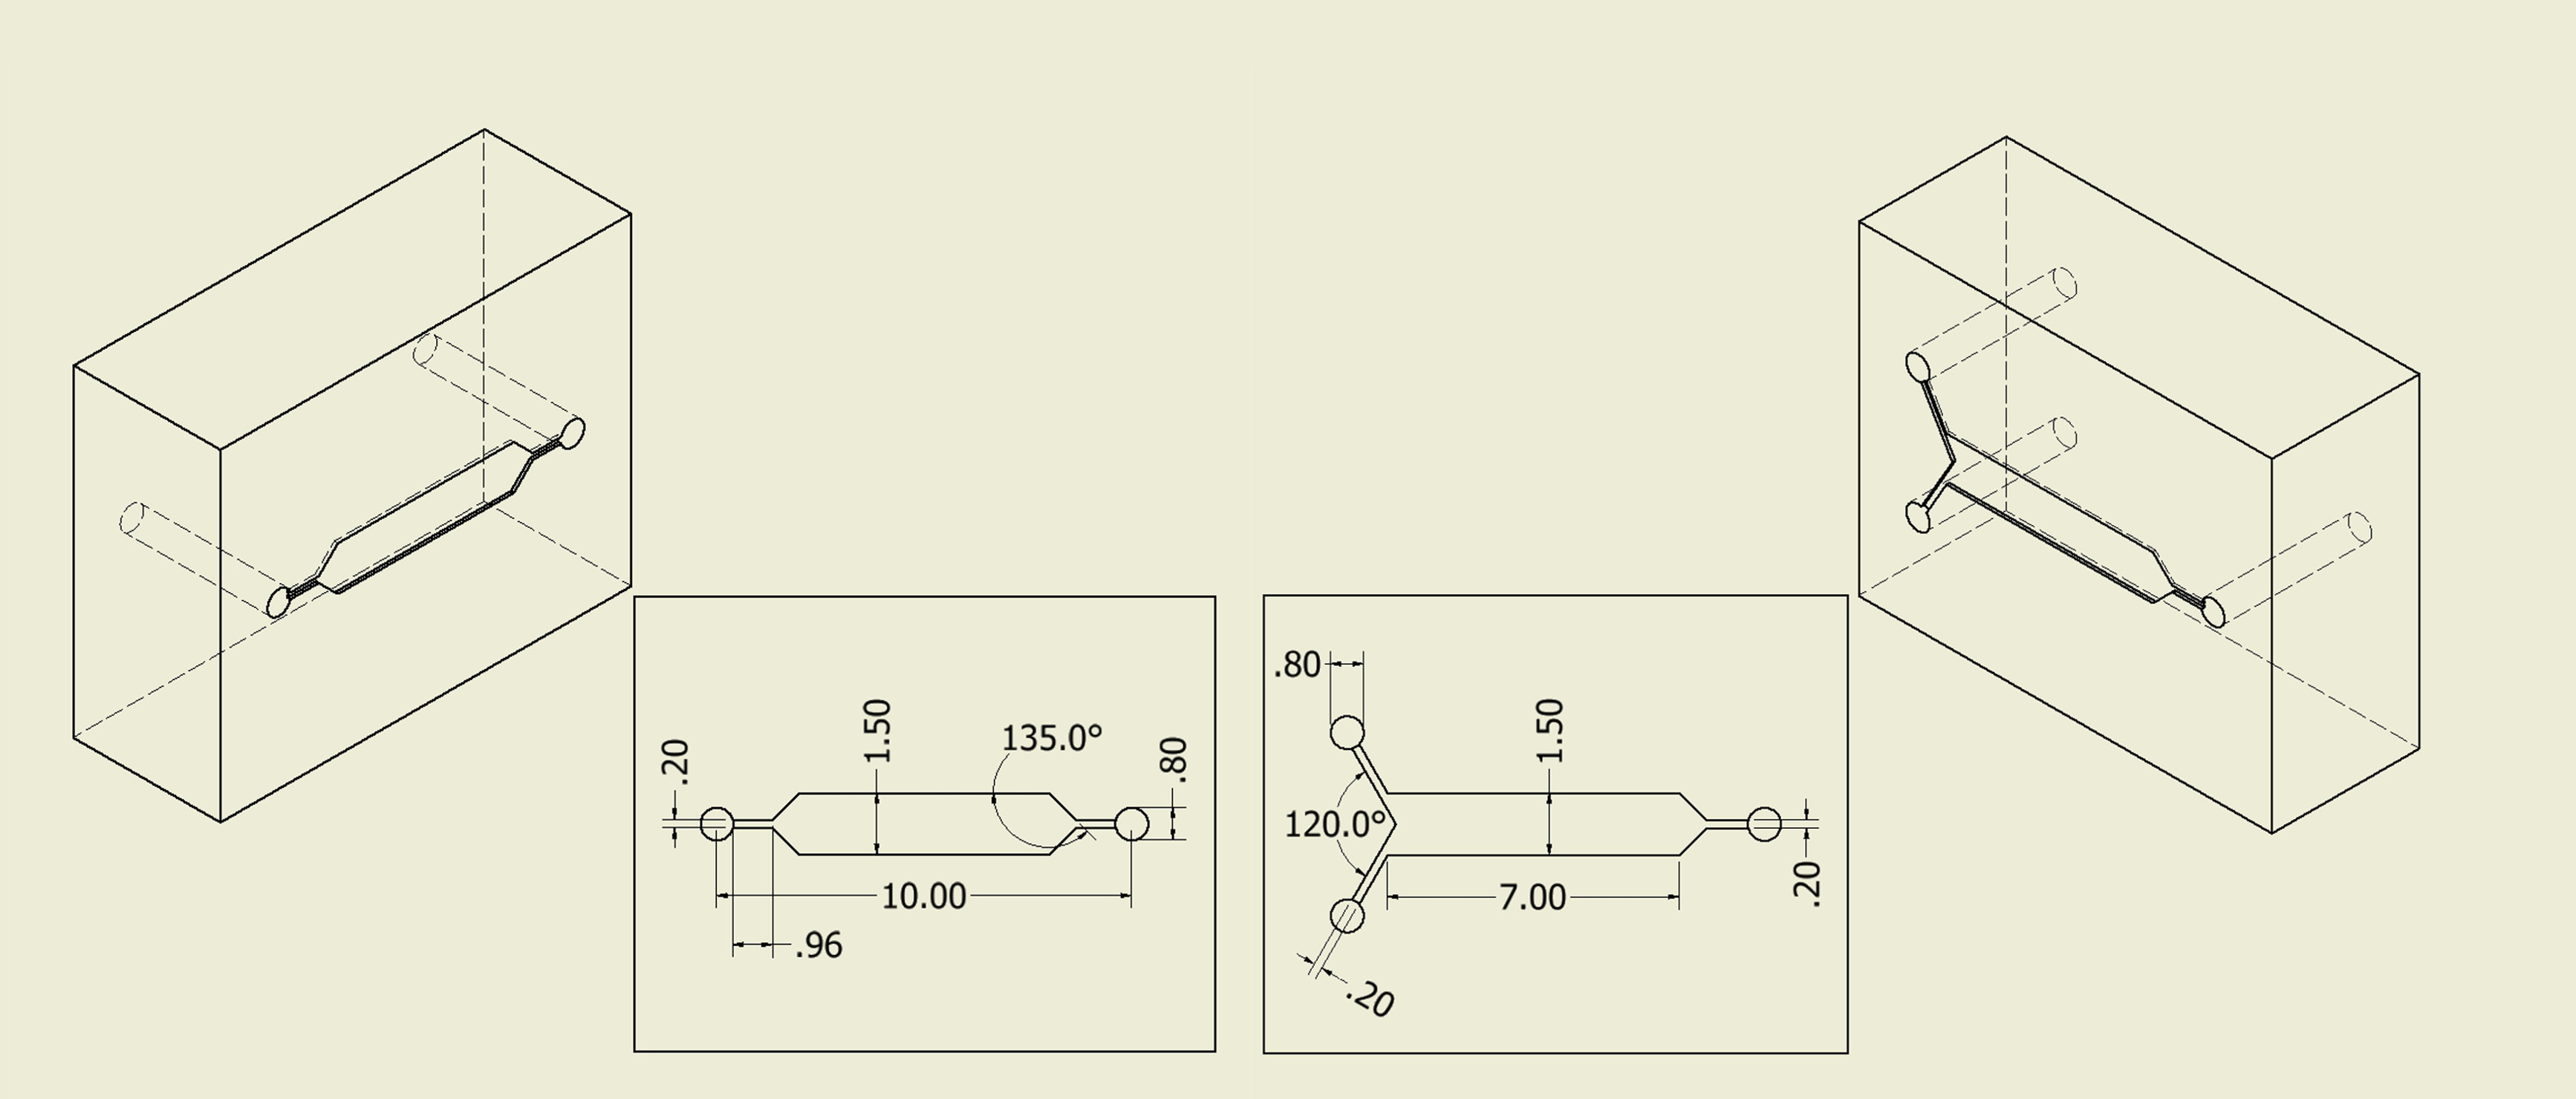
\includegraphics[width=14.5cm]{chapter4/figures/channelDimensions/dimensions.jpg}
            \caption[Schematics of the standard single layer microfluidic devices]{\textbf{Schematics of the standard single layer microfluidic devices.} All measurements listed in mm. Standard single layer microfluidic channels used in this section comprised both 2-port and 3-port (y-shaped) configuration.}
            \label{fig:devices:basicDimensions}
     \end{figure}



        \subsubsection{Evaporation and surface chemistry considerations}
        The initial incubation configuration explored was to apply a \(200 \mu L\) drop of media to the top of the PDMS surface to act as a media reservoir from which nutrients are exchanged and to preserve the aqueous environment. To minimize evaporation, the devices were further kept in a closed petri dish next to a dish with \(1 mL\) DDW. The petri dish was kept in a humidified CO\textsubscript{2} incubator (Figure \ref{fig:devices:osmIssue} A). The initial configuration also incorporated a 30 minute incubation with PLL solution as surface preparation. Cultures seeded in this configuration did not develop long term. The cells were initially healthy and adhered to the surface but the adhesion was non-uniform and by 5 days \textit{in vitro} the cultures degenerated (figure \ref{fig:devices:osmIssue} C-D). The main issue associated with this device configuration was that evaporation from the media on top of the devices was causing a rapid increase in the media osmolarity at a rate intolerable to the cells. We quantified this effect by measuring the osmolarity (Osmomat 030, Gonotec) of the media on top of 15 such devices after an overnight incubation. We found that the osmolarity drifted by \(126 \pm 97 mOsm\) overnight, implying an evaporation rate of \(49 \pm 20 \mu L\cdot day^{-1}\).

        \begin{figure}
           \centering
            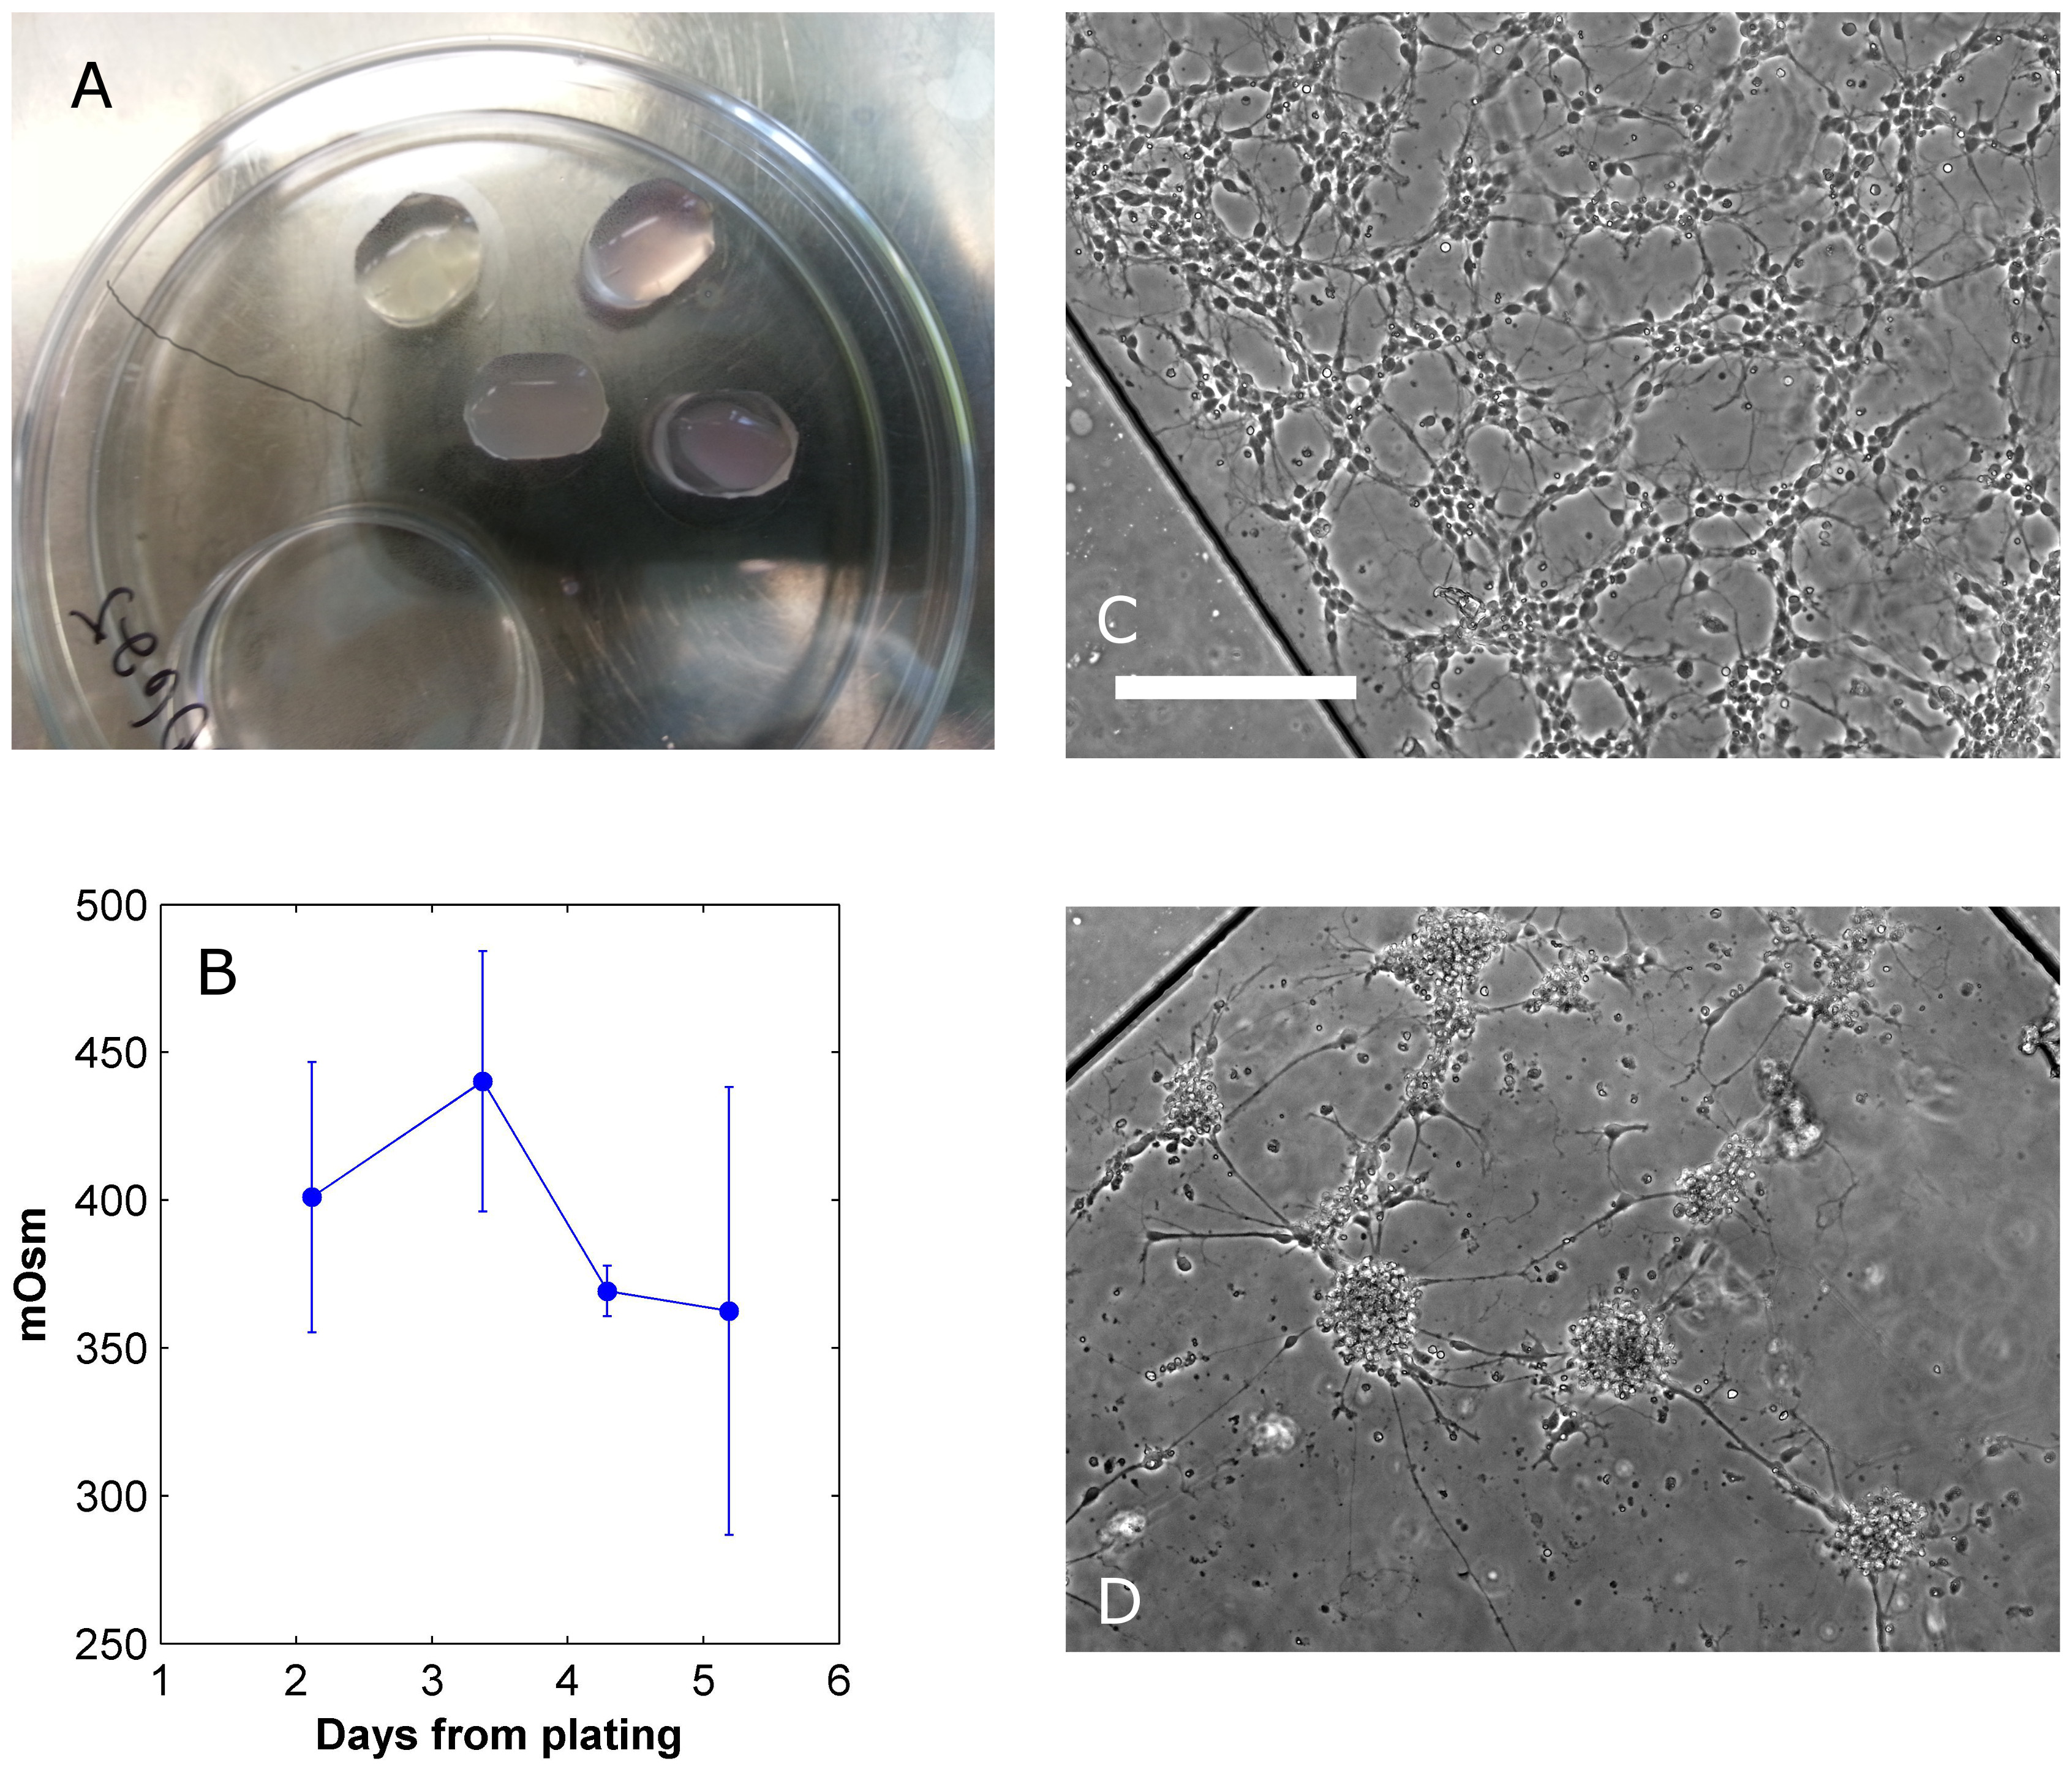
\includegraphics[width=14.3cm]{chapter4/figures/osmIssue/osmIssue.jpg}
            \caption[Effects of osmolarity drift in early protocol for long term culturing of neurons in microfluidic devices]{\textbf{The `drop on top' configuration results in excessive osmotic drifts and degeneration of the cultures.} (A) Top view of a group of devices illustrating the `drop on top' approach. (B) Osmolarity measurements taken from the drops on top of the devices in A during a maintenance protocol where the drop on top was changed every day. (C-D) Images of a culture growing in the `drop on top' configuration and where the drop was changed only twice weekly. Images are at 2 and 5 days \textit{in vitro}, respectively. By 5 days \textit{in vitro} the cell have aggregated and the glass surface remained relatively free of neurites and tissue, indicating degeneration (compare to figure \ref{fig:devices:tapeCultures} A,C which shows healthy cultures at the same age). Scale bar is \(200 \mu m\) long and is consistent for both images C and D.}
            \label{fig:devices:osmIssue}
        \end{figure}

        We tried to circumvent the evaporation issue by changing the drop on top of the devices every day (as opposed to twice weekly) and assessed the effectiveness by following the osmolarity of 4 devices for several days following the plating. Figure \ref{fig:devices:osmIssue} B shows that the osmolarity in this case was stable but still very high (values of \(\approx 400mOsm\) where as the osmolarity of our Neurobasal growth media is \(225 mOsm\)). A better solution was provided by switching to a maintenance routine where the devices were fully immersed in \(2.5-3 mL\) of culture media for the duration of the culture development (figure \ref{fig:devices:immersion}). Full details of this routine are provided in section \ref{sec:methods:culture}. The volumes of media applied to each sample in this approach are comparable to what is used in standard cell culture samples so media could be changed just twice a week without incurring excessive osmotic drifts. After 3 weeks of culturing in this approach, media osmolarity never drifted by more than \(30 mOsm\). Beyond this, the initial patchiness in adhesion led us to suspect that 30 minutes of PLL incubation, which is adequate for standard open surfaces, might be be insufficient in the case of microfluidic devices where the extreme surface to volume ratio might cause an increased flux of PLL molecules into the PDMS and reduce the effective concentration available for the glass surface. Consequently, we also modified the protocol to an overnight PLL incubation. With this modified protocol we were able to sustain neuronal cultures for long term (figure \ref{fig:devices:volDensIssue}) but still not ideally, as will be described in the next section.




        \subsubsection{Considerations of factor circulation}
        \label{sec:devices:circulation}
        \begin{figure}[!htb]
           \centering
            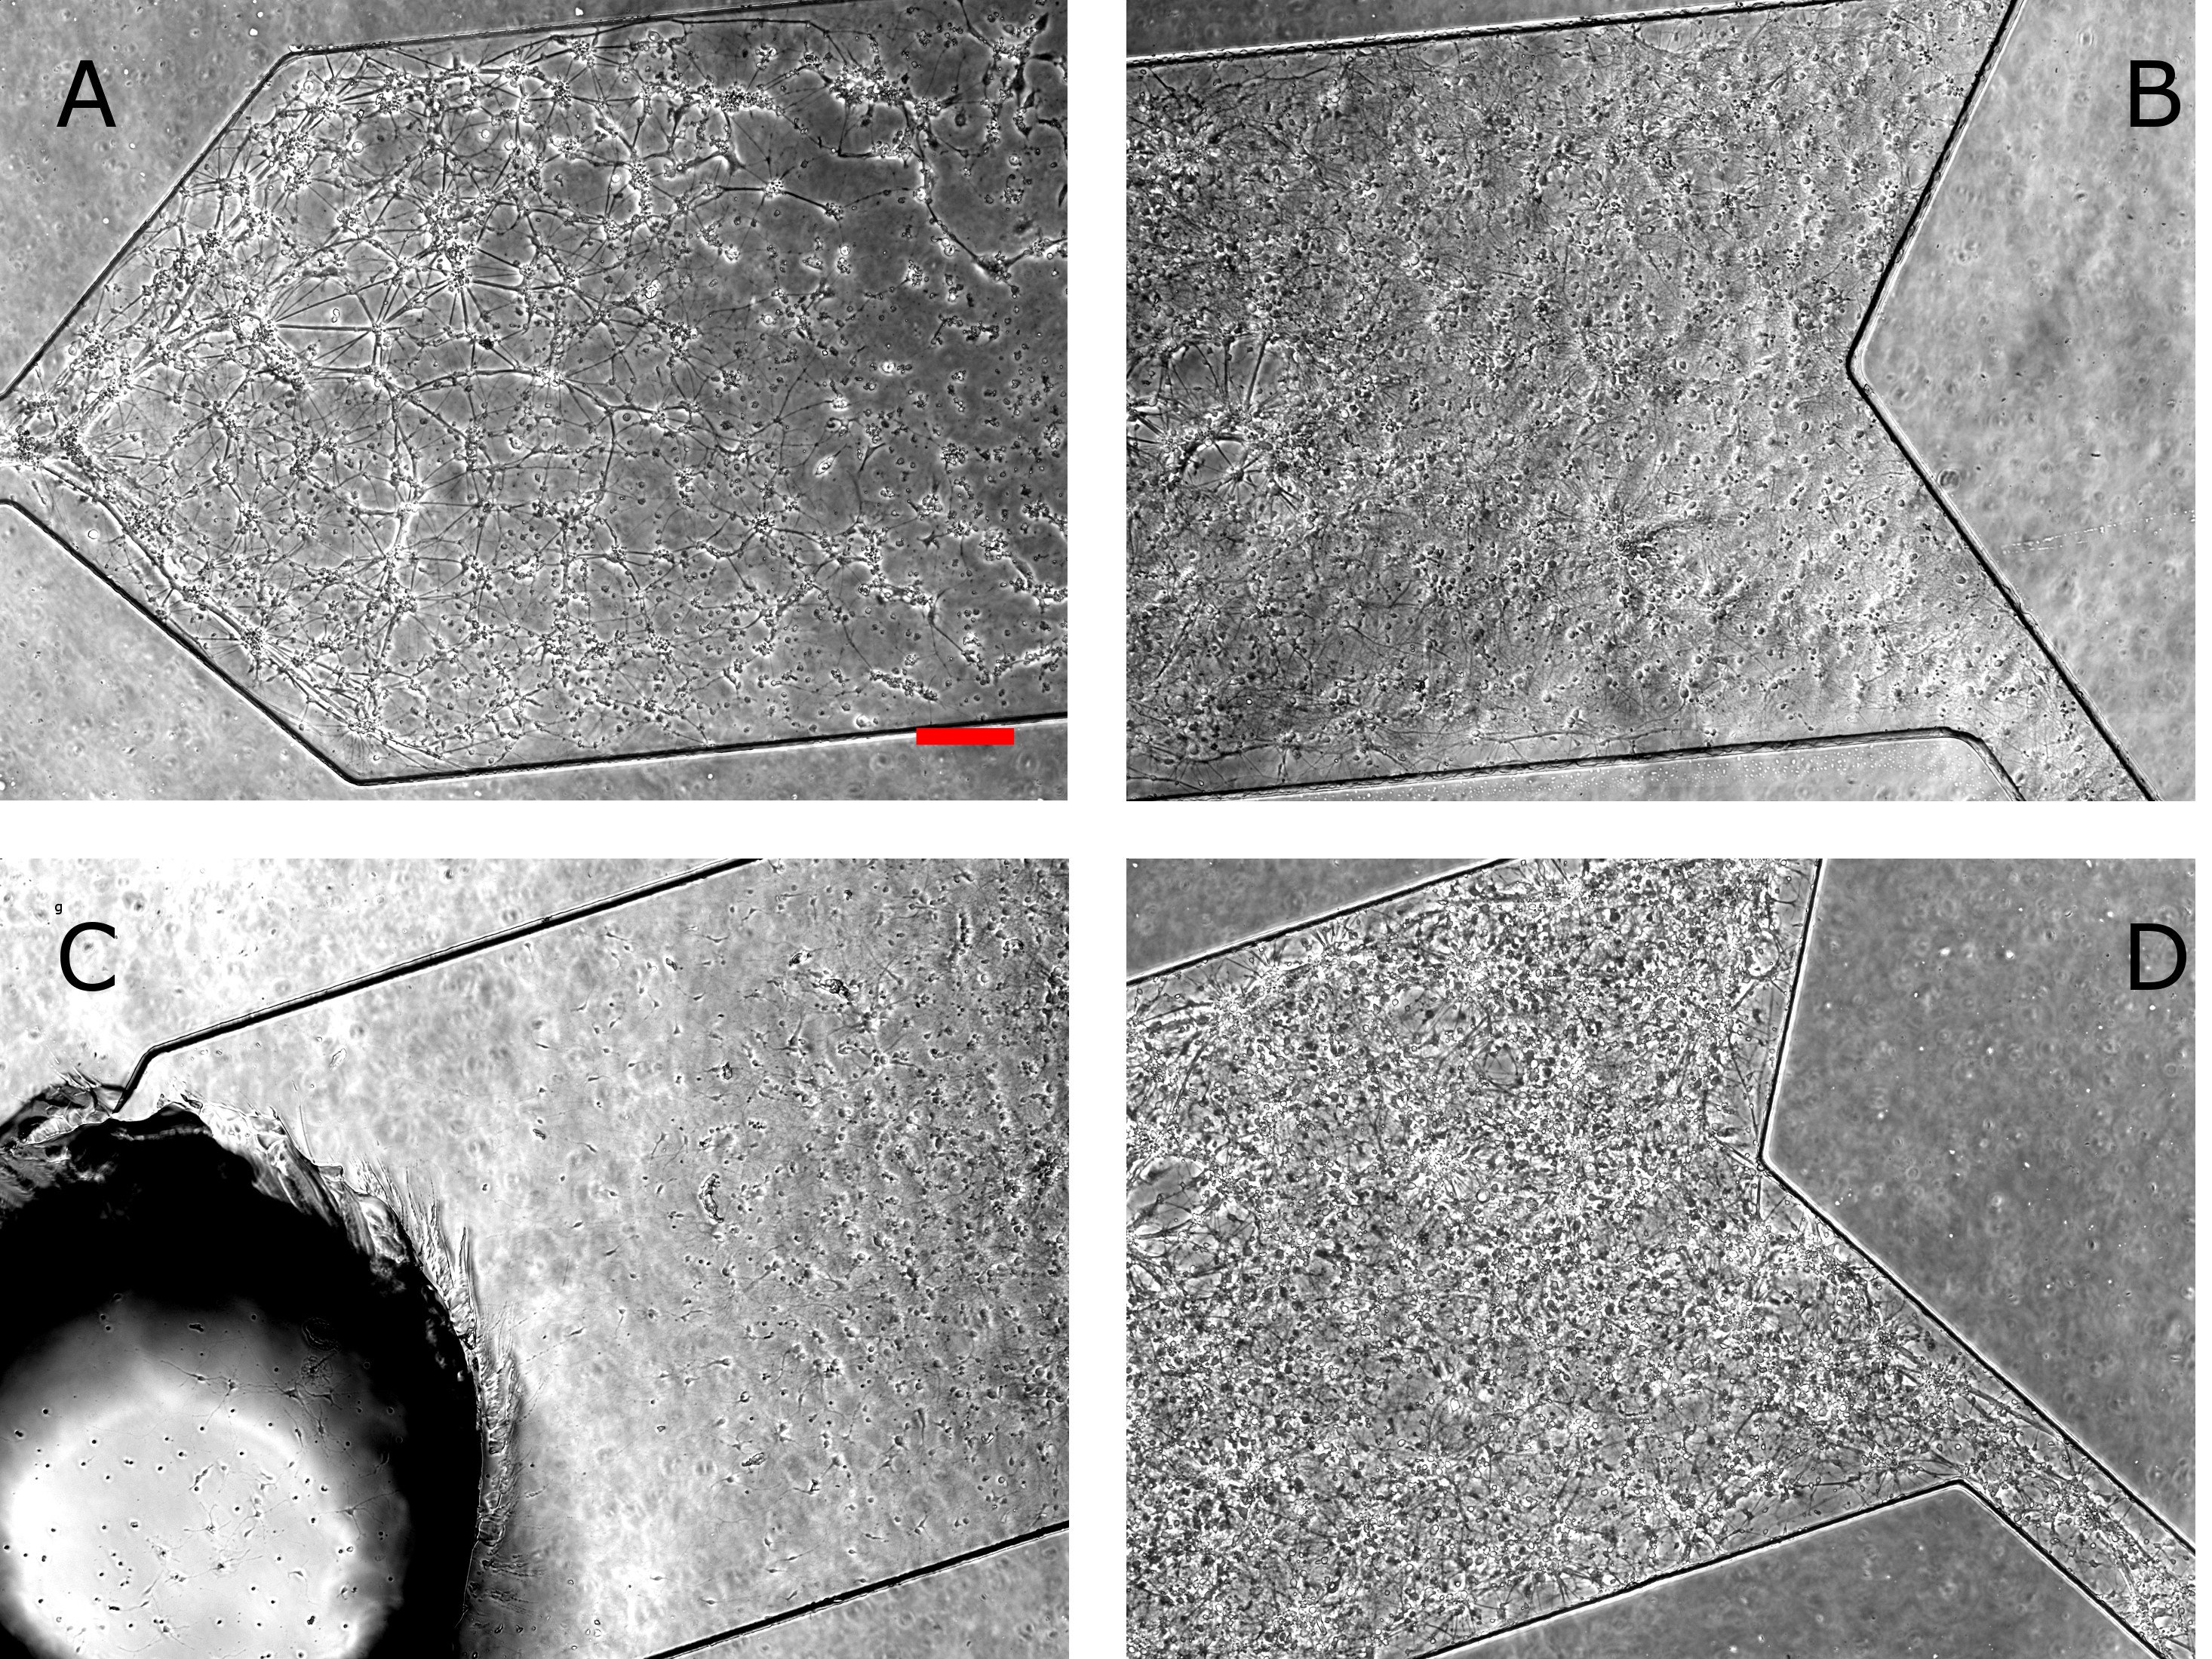
\includegraphics[width=12.4cm]{chapter4/figures/volDensIssue/volDensIssue.jpg}
            \caption[Demonstration of the limitations of circulation in planar microfluidic devices]{\textbf{A circulation bottleneck can emerge in microfluidic devices.} (A-B) Images of a culture growing in 3-port microfluidic devices where all the ports are \(0.8 mm\) in diameter. The images show the culture condition in the seeding port side and in the other side, respectively. Culture in the vicinity of the seeding port has degenerated, as indicated by the aggregation, prevalence of dead cells (observed as dots smaller then viable somata) and by the glass between the cells remaining bare. (C-D) Images of a culture growing in 3-port microfluidic devices where one of the ports is twice as big (\(1.6 mm\), indicated in red in the illustration). Images show culture condition in both sides of the device as before. Images were taken at 12 days \textit{in vitro}. Seeding solution density was of \(40\times10^6 cells\cdot ml^{1}\) which is equivalent to \(2600 cells\cdot mm^{-2}\) assuming homogenous distribution of the cells. Devices were maintained as described in section \ref{sec:methods:culture}. The location of imaging along the channel is indicated by the green rectangle in the illustration. Scale bar is \(200 \mu m\) long and is consistent across all images.}
            \label{fig:devices:volDensIssue}
        \end{figure}
        Figure \ref{fig:devices:volDensIssue} A-B shows microscope images of two sides of an example device 12 days after seeding during which it was maintained using the modified protocol as described above. The part of the culture residing in the vicinity of the seeding port did not develop properly and was mostly degenerated. Remarkably, the part of the very same culture residing on the side opposite to the seeding port was able to develop properly and maintain a healthy appearance for several weeks. A hint as to the mechanism operating behind the above phenomena comes from devices where one of the ports was punched to be twice as big (figure \ref{fig:devices:volDensIssue} C-D). In this case the cells were seeded from one of the ports opposite to the large port. In these large port devices the whole culture developed healthily without any significant spatial differences. Another clue was provided by our exploration of devices with a larger architecture where the height of the channel was \(1 mm\) and its internal volume \(\approx 20 \mu L\). The density of the plating solution for these devices was calculated so that the plated area density would be as in the small devices, \(2600 cells\cdot mm^{-2}\). Nevertheless, culture grown in these larger devices never exhibited any sign of such spatially arranged degeneration and typically developed well for several weeks. We hypothesised that the most likely explanation for the above observations is that the configuration of small devices and small ports does not provide adequate circulation to remove metabolic by-products and provide fresh nutrients to all parts of the culture. The fact that the degeneration occurred in proximity to the seeding port could be explained either by the port being blocked by lumps of cells or by a existence of a gradient of cell density along the channel. In both cases there would be a large unmet circulatory demand around the seeding port. In the case of the large port or the large devices, a stronger diffusive coupling between the culture and the external bulk media is enabled so in those cases circulation was not an issue. Since the configuration of small devices and small ports was required to properly interface with the flow tubing and to reach the required flow speeds we experimented with reduced plating densities in hope that these will have reduced circulatory demands. Indeed we found that by decreasing the plating density 6 fold (giving an area density of \(\approx 450 cells\cdot mm^{-2}\)) the spatially arranged degeneration phenomenon disappeared.

        The observations described in this section demonstrate how microfluidic technology can impose conditions that are not normally met in standard preparations. The area density of \(2600 cell\cdot mm^{-2}\) seeded in the earlier versions of the protocol is high but still commonly used for many applications involving neuronal culture. In those cases the culture is in immediate contact with a large volume of bulk media which readily supplies nutrients and removes by-products via diffusion. In our microfluidic devices, the internal volume of media is 3 orders of magnitude reduced (\(\approx 1 \mu L\)) and it is only in this extreme configuration that circulation becomes an issue. This situation is similar to cases where non-vascularized 3D cultures develop a necrotic core due to the lack of oxygen and nutrient penetration.

        \subsubsection{Alternative bonding methods}
        \label{sec:devices:bonding}
        Plasma bonding is a lengthy process that needs to be applied to each sample separately and therefore is not well suited for producing large quantities of devices. Additionally, it is not practical for more complex devices involving several layers as having to apply plasma bonding methodology to each layer separately makes the production of every single device very time consuming and error prone. Consequently, we experimented with alternative bonding approaches that have been recently suggested for assembly of microfluidic devices \cite{samel2007fabrication,nath2010rapid}. Complete protocols and illustrations are provided in section \ref{sec:methods:bonding}.

         \begin{figure}[h]
            \centering
            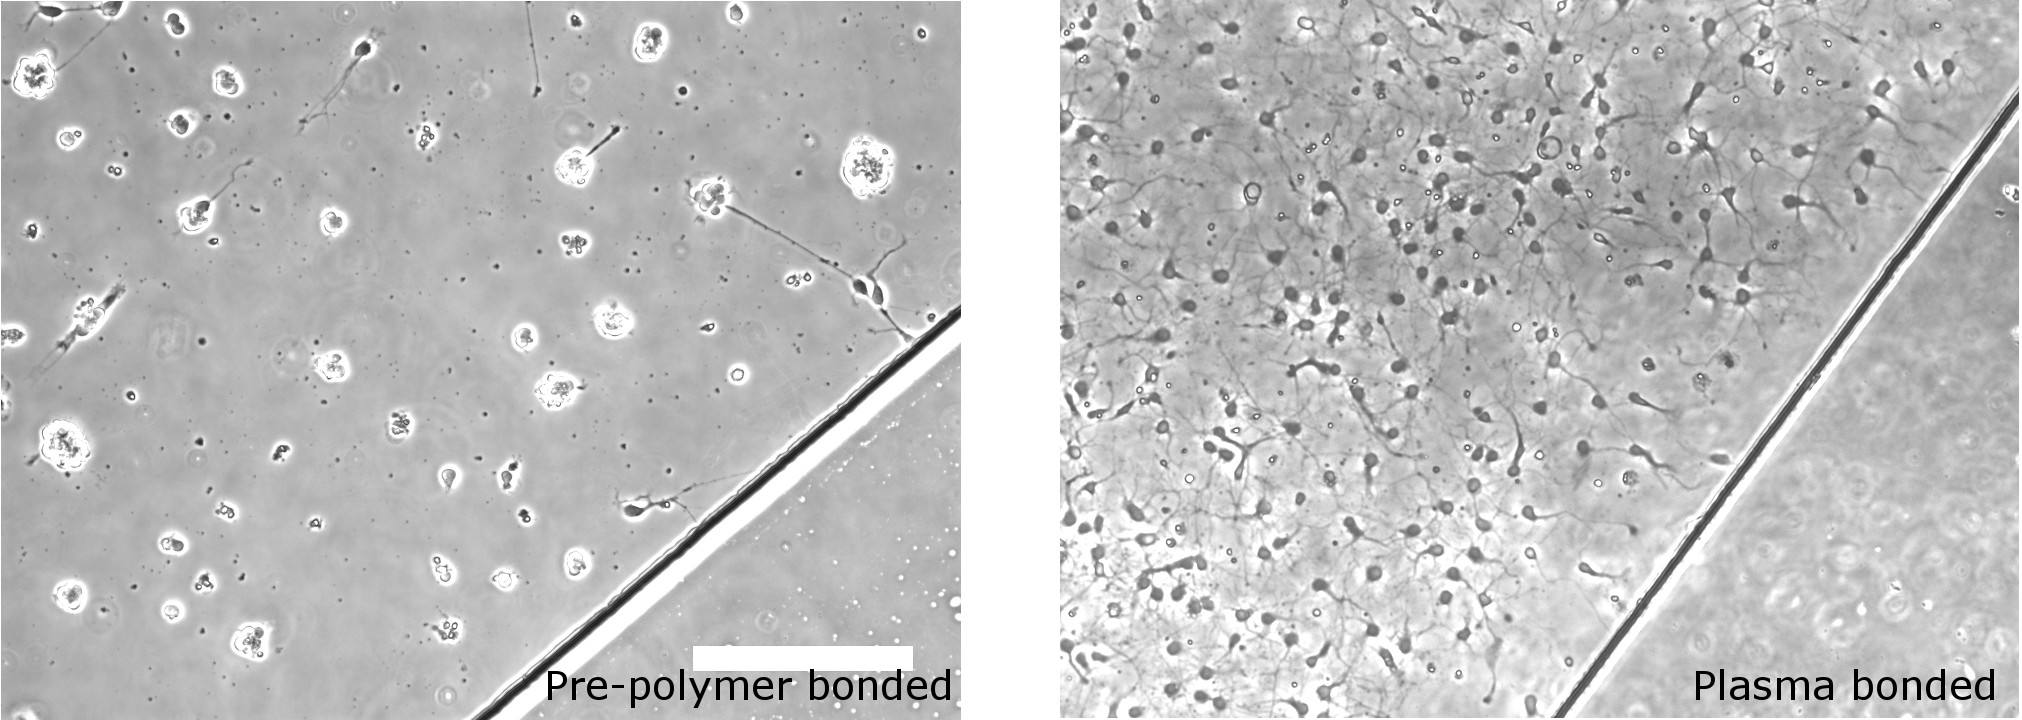
\includegraphics[width=15cm]{chapter4/figures/glueBonding/glueBondingComp.jpg}
            \caption[Effect of the pre-polymer bonding approach on the development of neuronal cultures in microfluidic devices]{\textbf{Contamination associated with pre-polymer bonding renders the surface unsuitable for neuronal adhesion.} Images comparing a culture growing in pre-polymer bonded devices to one growing in plasma bonded devices. The images were taken at 5 days \textit{in vitro}. Following bonding, the devices were subjected to identical surface preparation, seeding (density \(7\times10^6 cells\cdot ml^{-1}\)). and maintenance protocols (see sections \ref{sec:methods:surface} and \ref{sec:methods:culture}). Scale bar is \(200 \mu m\) long and is consistent across both images.}
            \label{fig:devices:glueBonding}
        \end{figure}


        The first approach attempted was to use the PDMS polymerization catalyst as an intermediate layer between the glass and PDMS bulk. The PDMS is dipped in catalyst solution, placed on top of the glass substrate and left to cure. This apparently induces further polymerization as well as partial covalent binding with the glass and results in a bond strength comparable or greater than plasma bonding \cite{samel2007fabrication}. We were able to achieve adequate bonding using this method but unfortunately the internal device surface proved to be completely inadequate for neuronal growth (figure \ref{fig:devices:glueBonding}. Interestingly, such a problem was not presented for other cell types such as astrocytes and HEK cells). This issue serves as another demonstration of the specific demands that are presented by neuronal culture. It is known that PDMS, when in contact with a surface, can contaminate the exposed areas around the point of contact through `leaching' of PDMS oligomers or curing agent molecules. Indeed it has been shown that PDMS sometime acts as a source of contamination interfering with neuronal growth inside microfluidic devices \cite{millet2007microfluidic}. The lack of adhesion reported here for the pre-polymer bound devices is probably an extreme manifestation of exactly these contamination processes.

        A different bonding alternative explored was that of using double sided silicone transfer tape \cite{nath2010rapid}. In this case channel features are not engraved into the PDMS through soft-lithography but simply cut out of the tape which is consequently joined with the glass surface. A square PDMS bulk with punched ports is joined to the top side of the tape to complete the body of the device. Since this method does not disrupt the surface coating of the non taped parts of the glass and can be performed in a sterile hood it opens the door for a new surface treatment approach. With tape based assembly the device can be taped to a pre-treated glass (surface-then-bond) whereas previously, with plasma bonding, the surface coating chemicals had to be introduced and incubated in the assembled device (bond-then-surface). This shift in paradigm allows to utilize the device geometry to control which parts of the treated surface will be exposed and available for culture adhesion and therefore offers an easy way of controlling its shape and size. This concept will be critical for the establishment of the microculture geometry in chapter \ref{chap:microculturePulses}.

        \begin{figure}[!htb]
            \centering
            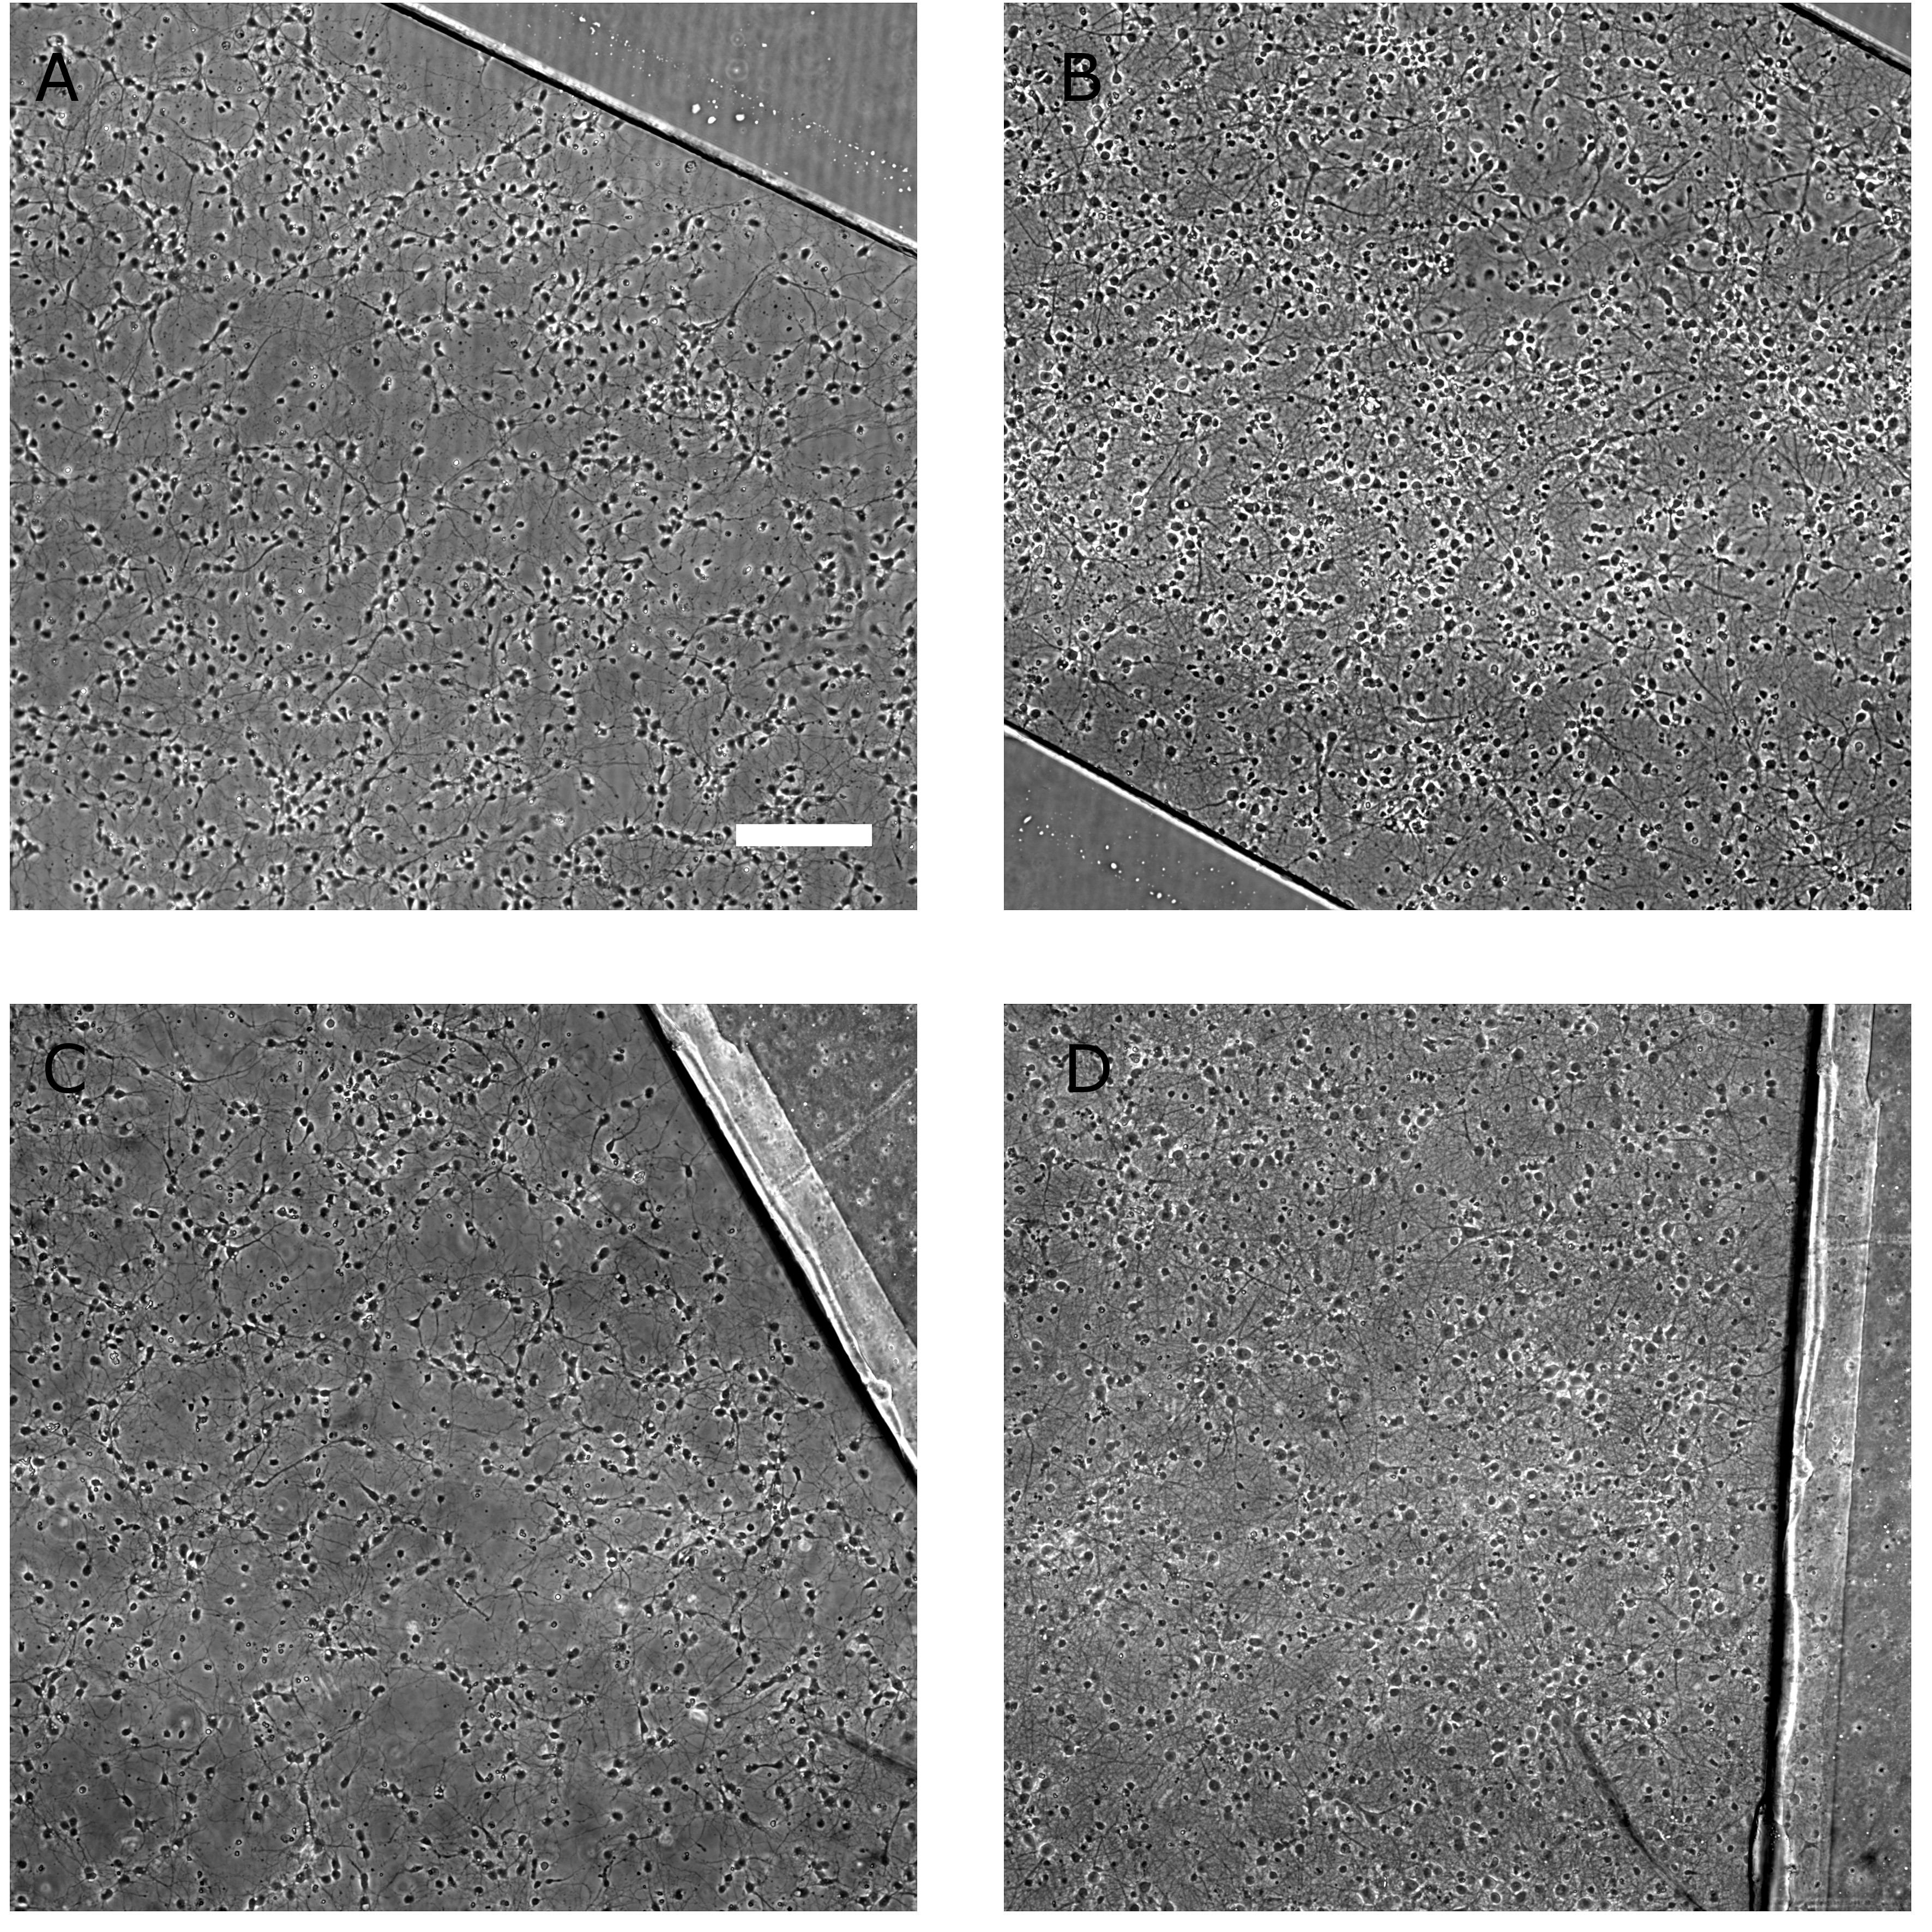
\includegraphics[width=15cm]{chapter4/figures/tapeCultures/tapeCultures.jpg}
            \caption[Comparison between cultures growing in plasma bonded devices and tape based devices]{\textbf{Tape based device architecture is fully compatible with neuronal culture.} (A-B) Cultures growing in plasma bonded devices at ages 5 and 12 days \textit{in vitro}, respectively. (C-D) Cultures growing in tape based devices at different stages of development as above. Plasma bonded devices were subjected to `bond-then-surface' surface preparation approach whereas tape based devices were subjected to `surface-then-bond' (see section \ref{sec:methods:surface}). Both devices were seeded and maintained as described in section \ref{sec:methods:culture}. Seeding density was \(7\times10^6 cells\cdot ml^{-1}\). Cultures in plasma bonded and tape devices are indistinguishable. Scale bar is \(200 \mu m\) long and is consistent across all images.}
            \label{fig:devices:tapeCultures}
        \end{figure}

        Figure \ref{fig:devices:tapeCultures} compares cultures grown in plasma bonded devices to ones grown in tape based and using the surface treatment paradigms appropriately as discussed above. The cultures are indistinguishable and appear to develop identically over the 12 days of inspection. This shows that the silicone tape is safe for use with neuronal culture and does not leach significant amount of toxins onto the surface or media. This tape based assembly approach will be cardinal for the multilayered devices described in chapters \ref{chap:activityAndFlow} and \ref{chap:microculturePulses}.


        \subsubsection{Extraction of PDMS}
        PDMS extraction is the last topic described with regards to the development of the basic protocol. As was apparent from the results of section \ref{sec:devices:bonding}, traces of curing agent or short oligomer chains can be harmful to neuronal cultures grown in the presence of PDMS. Indeed, even though the maintenance protocol achieved in section \ref{sec:devices:circulation} did generally sustain neuronal cultures for at a couple of weeks \textit{in vitro}, there were occasions where the cultures did not develop adequately. We reasoned that PDMS leaching might play a role in that inconsistency and therefore decided to try and employ a protocol for extraction of toxic species out of the cured devices. The protocol follows the suggestion from \cite{millet2007microfluidic} and is detailed in section \ref{sec:methods:fabrication}. Figure \ref{fig:devices:extraction} compares cultures grown in standard devices to those grown in extracted devices from the same plating and using the same maintenance protocol. In this plating, the cultures in standard devices seemed to fasciculate early on and completely degenerated by 12 days \textit{in vitro} (n=5). In the extracted devices (n=10) there was no sign of such degeneration. It should be noted that the extraction process involves immersing the devices in highly toxic solvents such as pentane and xylenes. When these are not properly oven-baked out of the devices a highly violent toxic effect is generated with the cells dying immediately upon seeding (figure \ref{fig:devices:extraction} C). Faulty development in non-extracted devices was not always observed and could be attributed to a specific PDMS mixing batch or to interactions with other factors. Nevertheless, to maximize the consistency of the preparations we added PDMS extraction to the standard protocol.

        \begin{figure}[!htb]
            \centering
            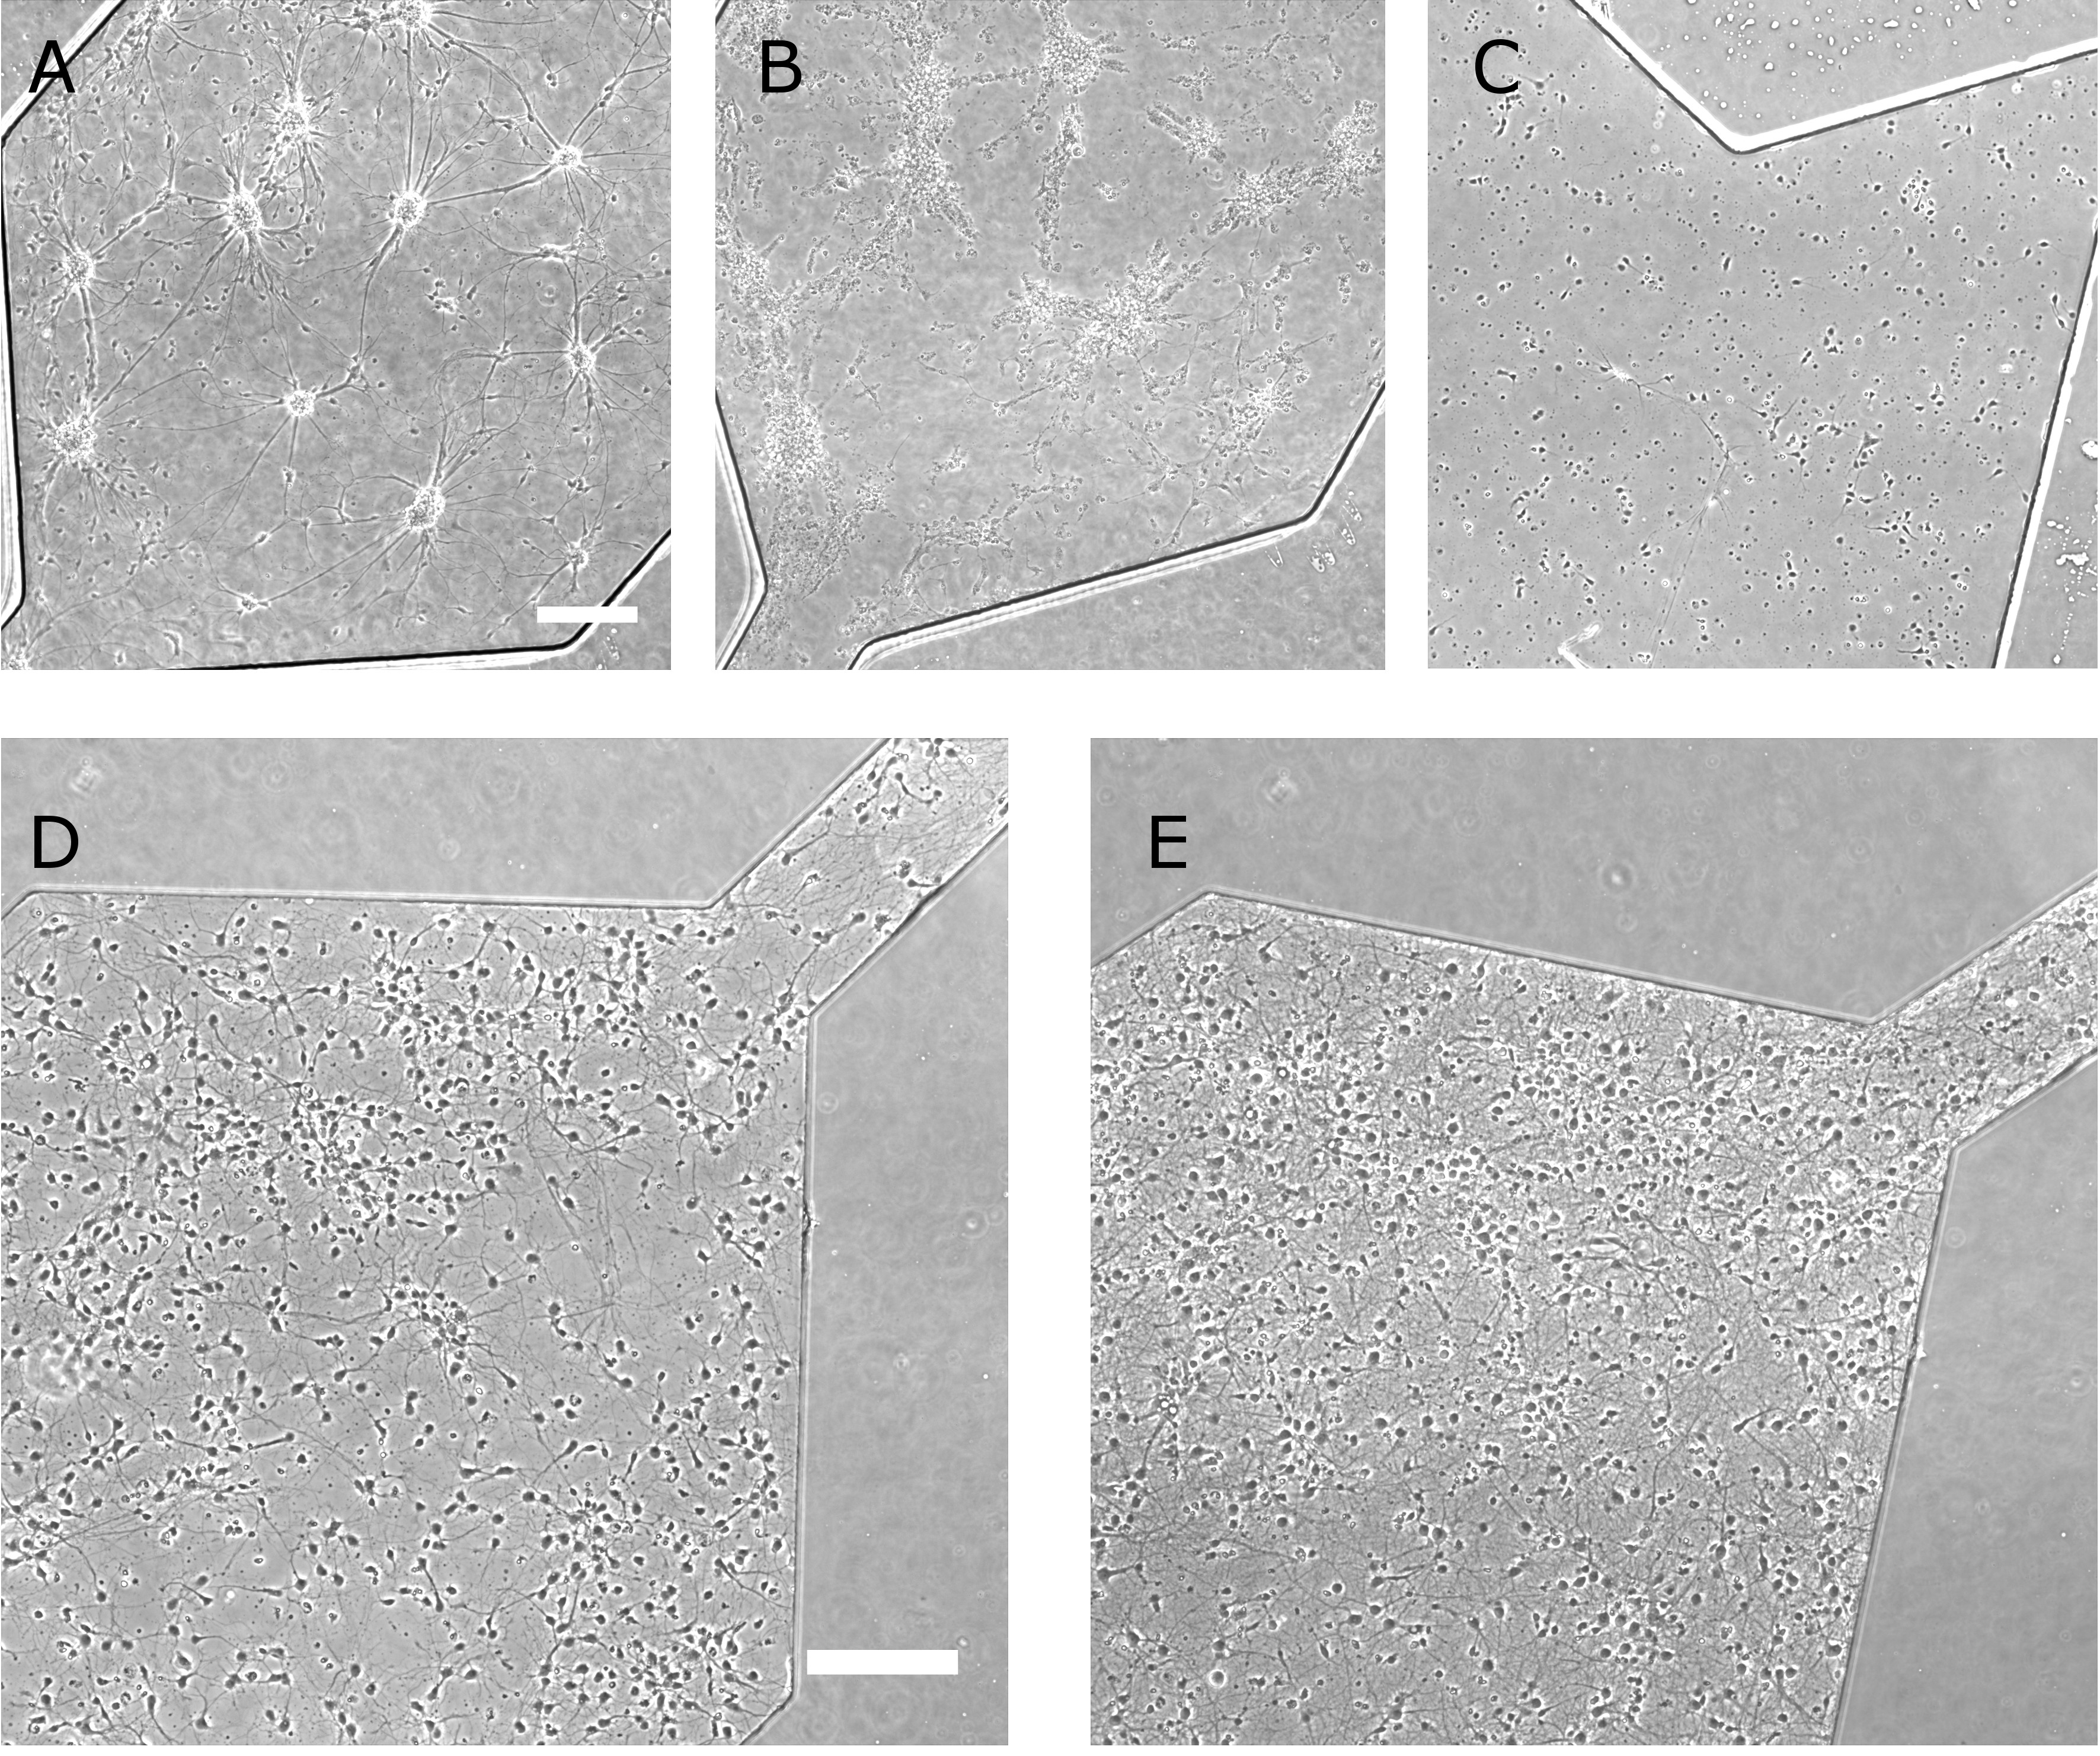
\includegraphics[width=15cm]{chapter4/figures/extraction/extractionIssue.jpg}
            \caption[Demonstration of PDMS related contaminations and the extraction procedure]{\textbf{Non extracted PDMS devices can leach out chemicals that are harmful to neuronal growth.} (A-B) Neuronal culture exhibiting adhesion and development issues that are thought to arise from PDMS leaching. Same culture is shown at ages 5 and 12 days \textit{in vitro}, respectively. (C) Culture seeded in a device made from extracted PDMS which was not baked long enough for removal of noxious extraction chemicals. Image was taken at 2 days \textit{in vitro}. (D-E) Cultures grown in extracted PDMS devices at 5 and 12 days \textit{in vitro}, respectively. These images represent the typical cultures achieved for the final protocol incorporating all the principles discussed in this section. All devices were plasma bonded (section \ref{sec:methods:fabrication}), subjected to `bond-then-surface' surface preparation (section \ref{sec:methods:surface}), seeded at a density of \(7\times10^6 cells\cdot ml^{-1}\) and maintained according to section \ref{sec:methods:culture}. Scale bar is \(200 \mu m\) long and is consistent across all images.}
            \label{fig:devices:extraction}
        \end{figure}

        To summarize, we have developed a protocol for long term growth of neuronal culture in planar (1-layer) microfluidic devices. We reviewed what we consider to be the important factors in the development of such protocols, namely, osmolarity, circulation of nutrients and oxygen, ease of assembly and leaching of chemicals from the construction materials (usually PDMS). Full details of the final protocol are provided in section \ref{sec:methods:culture}. This protocol is the basis for all the subsequent device types used in this Ph.D thesis. All of them will use the same preparation and maintenance routines and will differ only in the seeding density and volume which require adaptation to the specific device and culture geometry.

        \subsection{Growing microcultures in plasma bonded devices}
        \label{sec:devices:microcultures}

        As explained in section \ref{sec:devices:introduction}, controlling the physical extent of the culture is necessary in order to apply the interface shifting method in a way that produces physiologically relevant concentration pulses. Here we describe confinement of the cultures into microwells of a desired size. To add microwells to our device geometry, we produced a PDMS sheet with rectangular holes via thin film spinning on a silicon/SU-8 mold comprising pillars in the shape of the required microwells (see section \ref{sec:methods:fabrication}). To assemble the devices, the PDMS sheet was placed on a glass coverslip forming a reversible hydrophobic bond. The PDMS bulk with the engraved channel (as in figure \ref{fig:devices:basicDimensions}) was then plasma bonded to the PDMS sheet while being manually aligned to position the microwell within the channel borders (figure \ref{fig:devices:lithoMWell}). The devices were seeded at density of \(20\times10^6 cells\cdot ml^{-1}\) and volume of \(2 \mu L\). The seeding filled the entire device volume with cells which settled arbitrarily on the exposed PDMS or inside the microwells. After the initial seeding the devices were inspected under the microscope to check if there is adequate inhabitation of the microwells and subjected to flushing and re-seeding as necessary. As shown in figure \ref{fig:methods:mwProfile}, an undesirable side effect of the way the PDMS sheet was manufactured is that the microwells are produces with an elevated ridge around them. The ridge caused a directing of the cells around the microwells rather than into them which was the main reason why flushing and re-seeding was necessary at times. After obtaining adequate microwell inhabitation, the devices were left in the incubator for 2-3 hours for initial adhesion of the cells, then media was pulled through with a \(1 ml\) syringe. This pulling had a differential effect on the cells depending on their location, i.e., most of the cells on the PDMS surface were ripped off and removed by the pulling whereas the cells in the wells tended to stay put as they were protected from the shear. In this way, isolated neuronal microcultures were generated and they were maintained as described in section \ref{sec:methods:culture}.


        \begin{figure}[h]
            \centering
            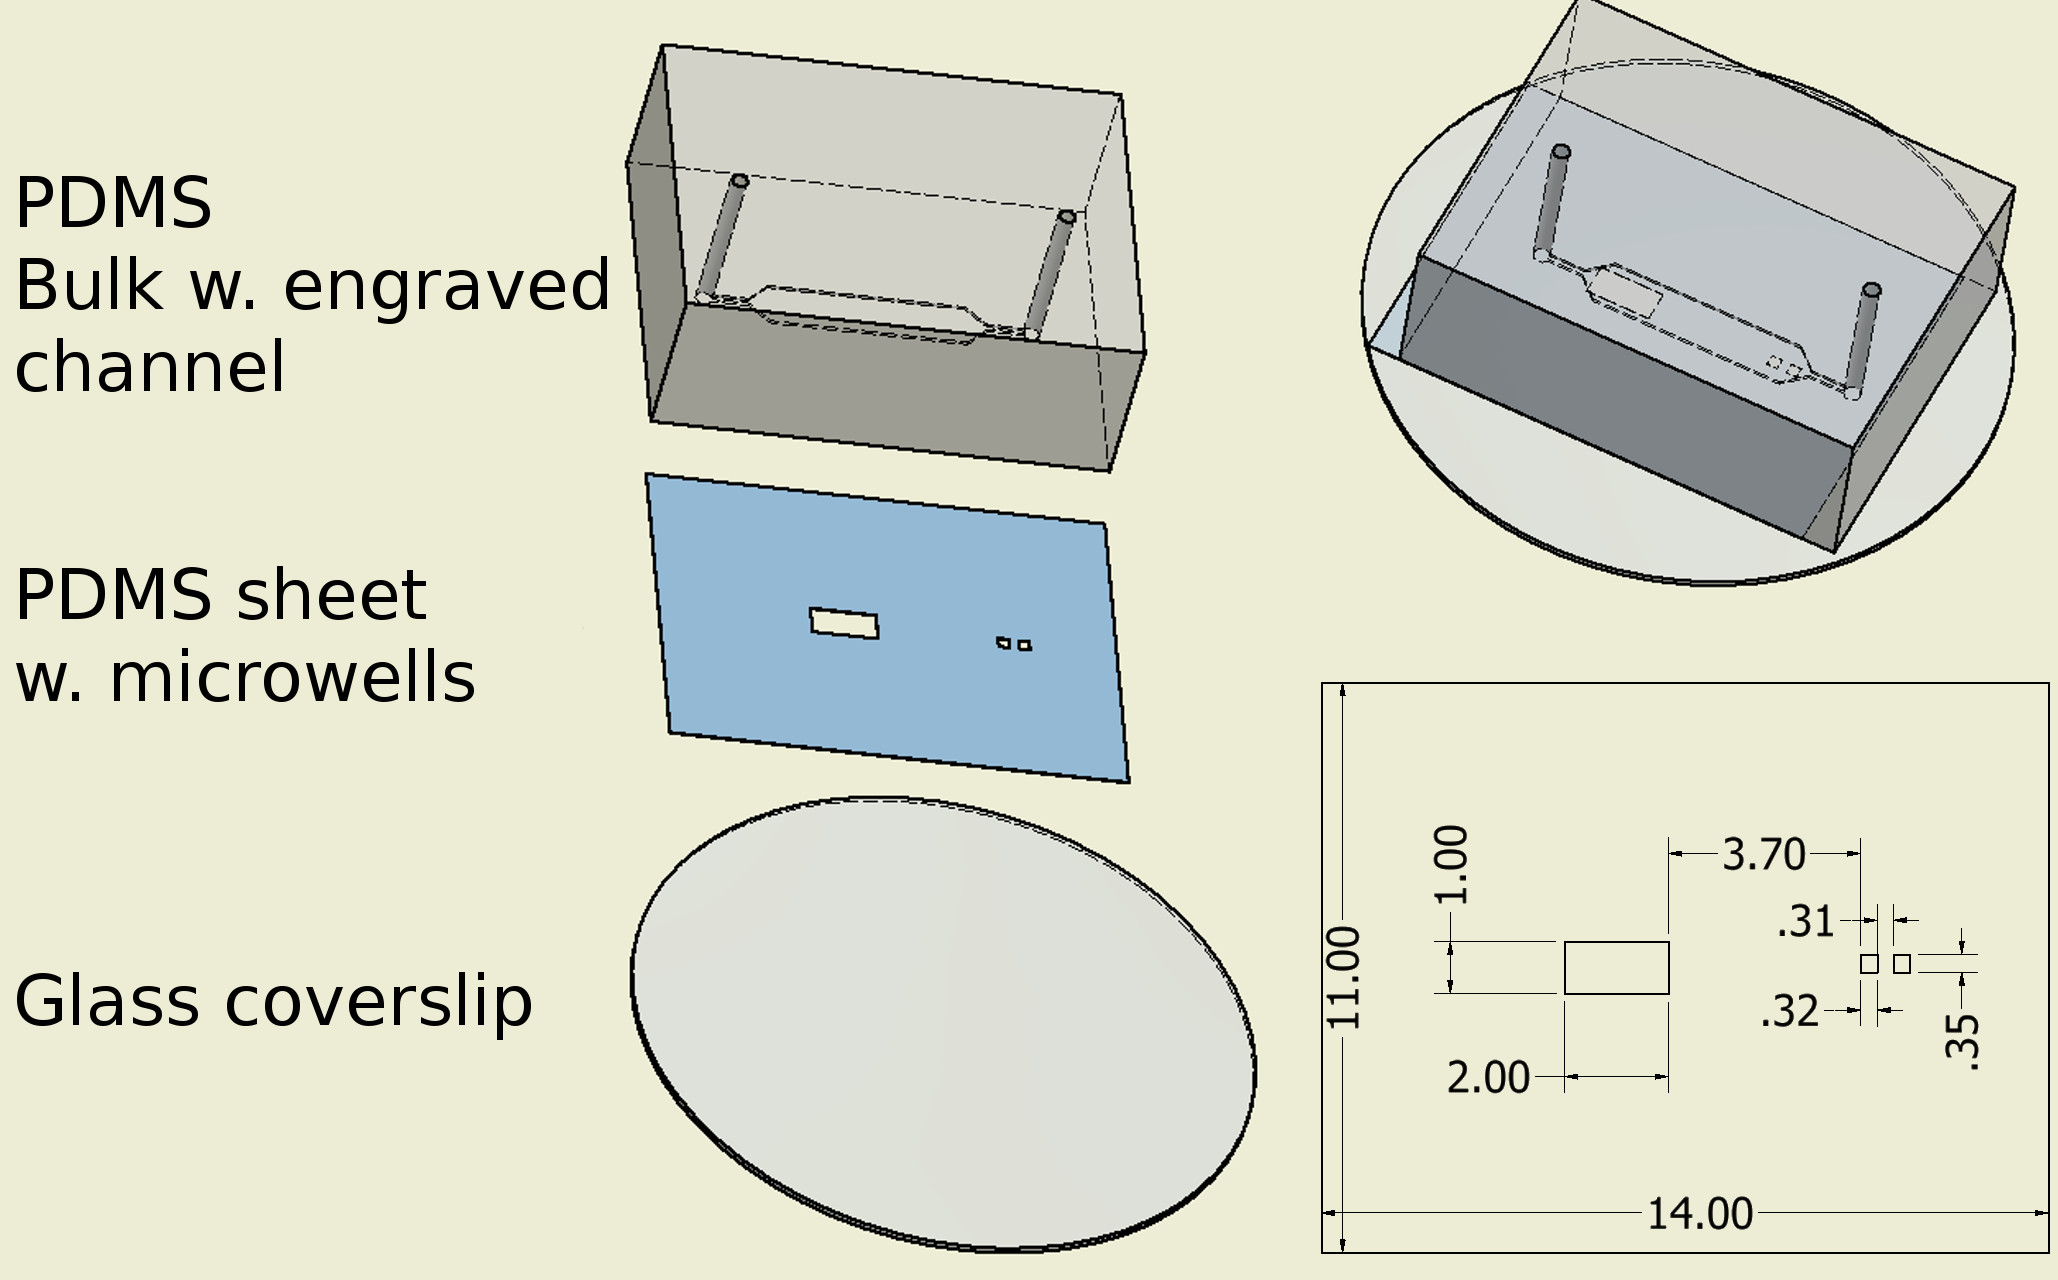
\includegraphics[width=7cm]{chapter4/figures/lithoMWell/lithoMWell.jpg}
            \caption[Schematics of the 2-layered microfluidic devices with microwells]{\textbf{Schematics of the 2-layered microfluidic devices with microwells.}
            The three components (PDMS bulk with an engraved microchannel, PDMS sheet and coverslip glass) of the device are shown separately and after bonding to illustrate how the the microwells are aligned to be within the channel boundaries. Dimensions of PDMS sheet are also presented in mm units. In this case, the microwells were of size \(350\times320 \mu m^2\). Dimensions of microchannel are as in figure \ref{fig:devices:basicDimensions}.}
            \label{fig:devices:lithoMWell}
        \end{figure}
        Section \ref{sec:devices:circulation} highlighted how, due to the small internal volume and narrow ports, our microfluidic devices can limit nutrient and oxygen circulation to the extent that necrosis is induced. In the case of the microcultures, however, the opposite extremity of factor circulation seemed to present itself. Initial attempts to grow microcultures under the aforementioned maintenance protocol resulted in the cells showing an initially good adhesion but failing to show any subsequent development and degenerating altogether by 5 days \textit{in vitro} (figure \ref{fig:devices:noSupport}). This degeneration was similar in time scales to the one caused by the osmotic drift but seemed to be more aggressive as the cells did very little even in the direction of initial sprouting of neurites. This type of degeneration is known to occur in small / low density cultures even in standard preparations (i.e., open surfaces, not microfluidic devices) \cite{kaech2006culturing} where it is presumed that the neurons are not able to generate a sufficient concentration of conditioning factors around them to sustain their development. The typical solution in this situation is to grow the cultures in proximity to a large pure astrocyte culture which shares the same media and secretes the required conditioning factors. This auxiliary astrocyte culture is sometime termed support culture. We followed this approach by adding two levels of support culture. One was harboured in a large well situated within the device several millimeters away from the microcultures (see figure \ref{fig:devices:lithoMWell}). A second one was a large culture plated outside the devices on the bare cover slip glass around the PDMS bulk. We found that the presence of these support cultures indeed prevented the aforementioned degeneration (figure \ref{fig:devices:mwDev}) and that both of them together were required for best results. We did not attempt growing pure astrocyte cultures for this as regular cortical cultures (which contain astrocytes) seemed sufficient to produce a beneficial effect.

        \begin{figure}[h]
            \centering
            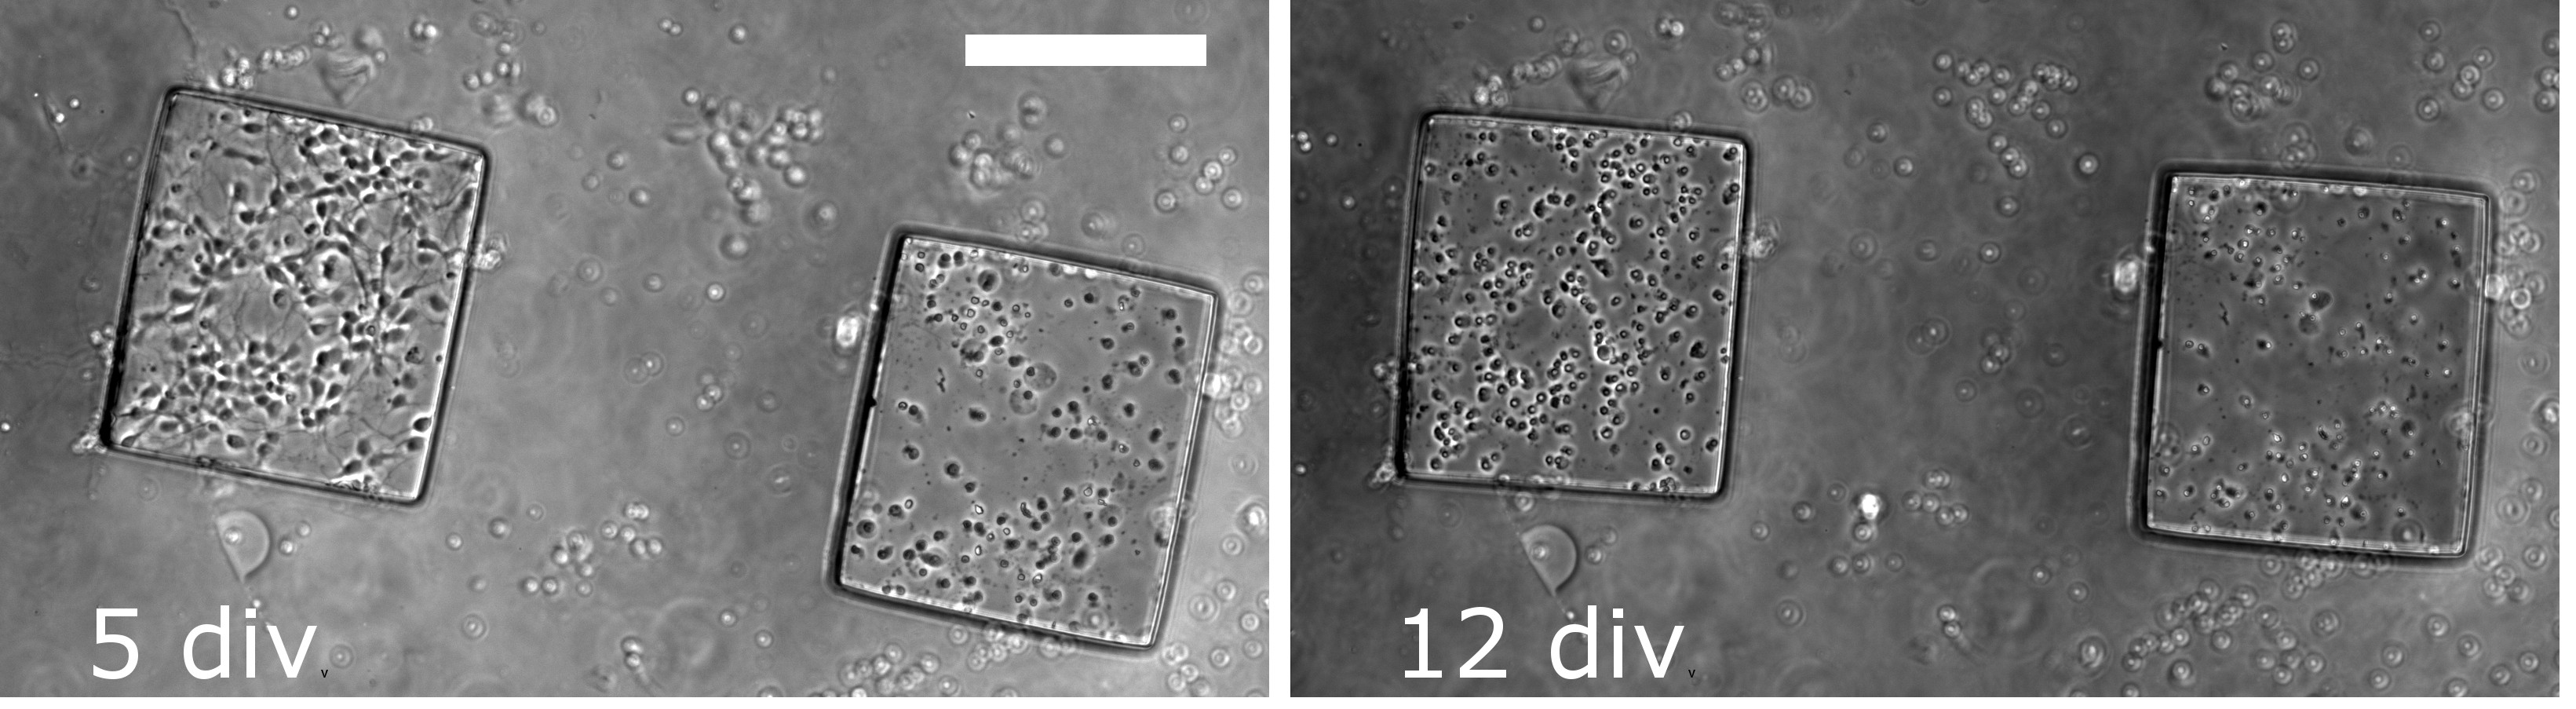
\includegraphics[width=13.8cm]{chapter4/figures/noSupport/noSupport.jpg}
            \caption[Neuronal microcultures growing without a support culture]{\textbf{Neuronal microcultures do not develop without a support culture.} Representative images of microcultures developing without seeding a support culture outside the device. The microwells were of size \(300\times270 \mu m^2\). Scale bar is \(200 \mu m\) long and is consistent across both images.}
            \label{fig:devices:noSupport}
        \end{figure}

        \begin{figure}[h]
            \centering
            \includegraphics[width=13.7cm]{chapter4/figures/microWellsDev/microwellsDev.jpg}
            \caption[Development of neuronal microcultures]{\textbf{Development of neuronal microcultures.} (A-B) Images of a neuronal microculture growing in a microwell of size \(400\times370 \mu m^2\) at 5 and 12 days \textit{in vitro}. (C-D) Images of two neuronal microcultures at developmental stages as above in microwells of size \(220\times190 \mu m^2\). Microcultures were seeded at a density of \(20\times10^6 cells\cdot ml^{-1}\), flushed and maintained as described in section \ref{sec:methods:culture}. Scale bar is \(200 \mu m\) long and is consistent across all images.}
            \label{fig:devices:mwDev}
        \end{figure}

        Since such microcultures are not a standard neuroscience model preparation and it is unknown what is the smallest size they can be made while still developing properly, we decided to conduct a quantitative examination of their viability. To that end, we designed devices with 3 different microwell sizes and followed their development over 12 days \textit{in vitro}. We counted the number of healthy cells in bright field images taken at 1, 5, 12 days \textit{in vitro} and calculated the proportion of cells dying between consecutive counting time points. This data are presented in figure \ref{fig:devices:mwStats} as a function of the density of cells in the well at the preceding time point and grouped by well size. This is compared to the same statistic computed in the same way for images of the standard cultures from section \ref{sec:devices:protocolDev} referred to here as macrocultures. It is evident from figure \ref{fig:devices:mwStats} A that, regardless of microwell size, the microculture death rates are strongly and negatively correlated with their density. This was corroborated with a linear regression analysis giving a statistically significant linear correlation (F-test, \(p=2\times10^{-4}\)). The macrocultures did not show such a density associated death rate (F-test, \(p=0.26\)) but the macroculture densities were much less variable so the analyzed density range was smaller. The averaged death rates of the macro- and microcultures are compared in figure \ref{fig:devices:mwStats} B. Microcultures of all 3 sizes exhibited a significantly higher death rate than the macrocultures (unbalanced t-test, \(p=2\times10^{-5}, 0.0012, 0.0027\) for well edge sizes \(200,300,400 \mu m\), respectively).

        Since microculture densities appeared to be a key factor in their long term viability we also performed a similar comparison with the microculture data restricted just to densities higher than \(1500 cells\cdot mm^{-2}\). This density threshold was selected because the data beyond it did not show a density dependent trend which meant that the beneficial effects were saturated. Indeed the death rates at such high density microcultures were reduced and the large \(400 \mu m\) ones exhibited death rates indistinguishable from those in macrocultures (unbalanced t-test, p=0.23). Smaller high density microcultures of sizes \(200\) and \(300 \mu m\) still showed a significantly larger death rate (unbalanced t-test, p=0.0012 and 0.0012, respectively).

        The above data are consistent with the notion that neuronal cultures need to generate an environment of conditioning factors around the cells to support their own development. Since this environment comprises secreted factors its buildup would strongly depend on the density and the size of the culture. Indeed the effect of both of these parameters is evident in the data shown here and a practical heuristic emerges that microcultures larger then \(400\times400 \mu m^2\) and denser than \(1500 cell\cdot mm^{-2}\) have a potential of developing as well as macrocultures.

        \begin{figure}[h]
            \centering
            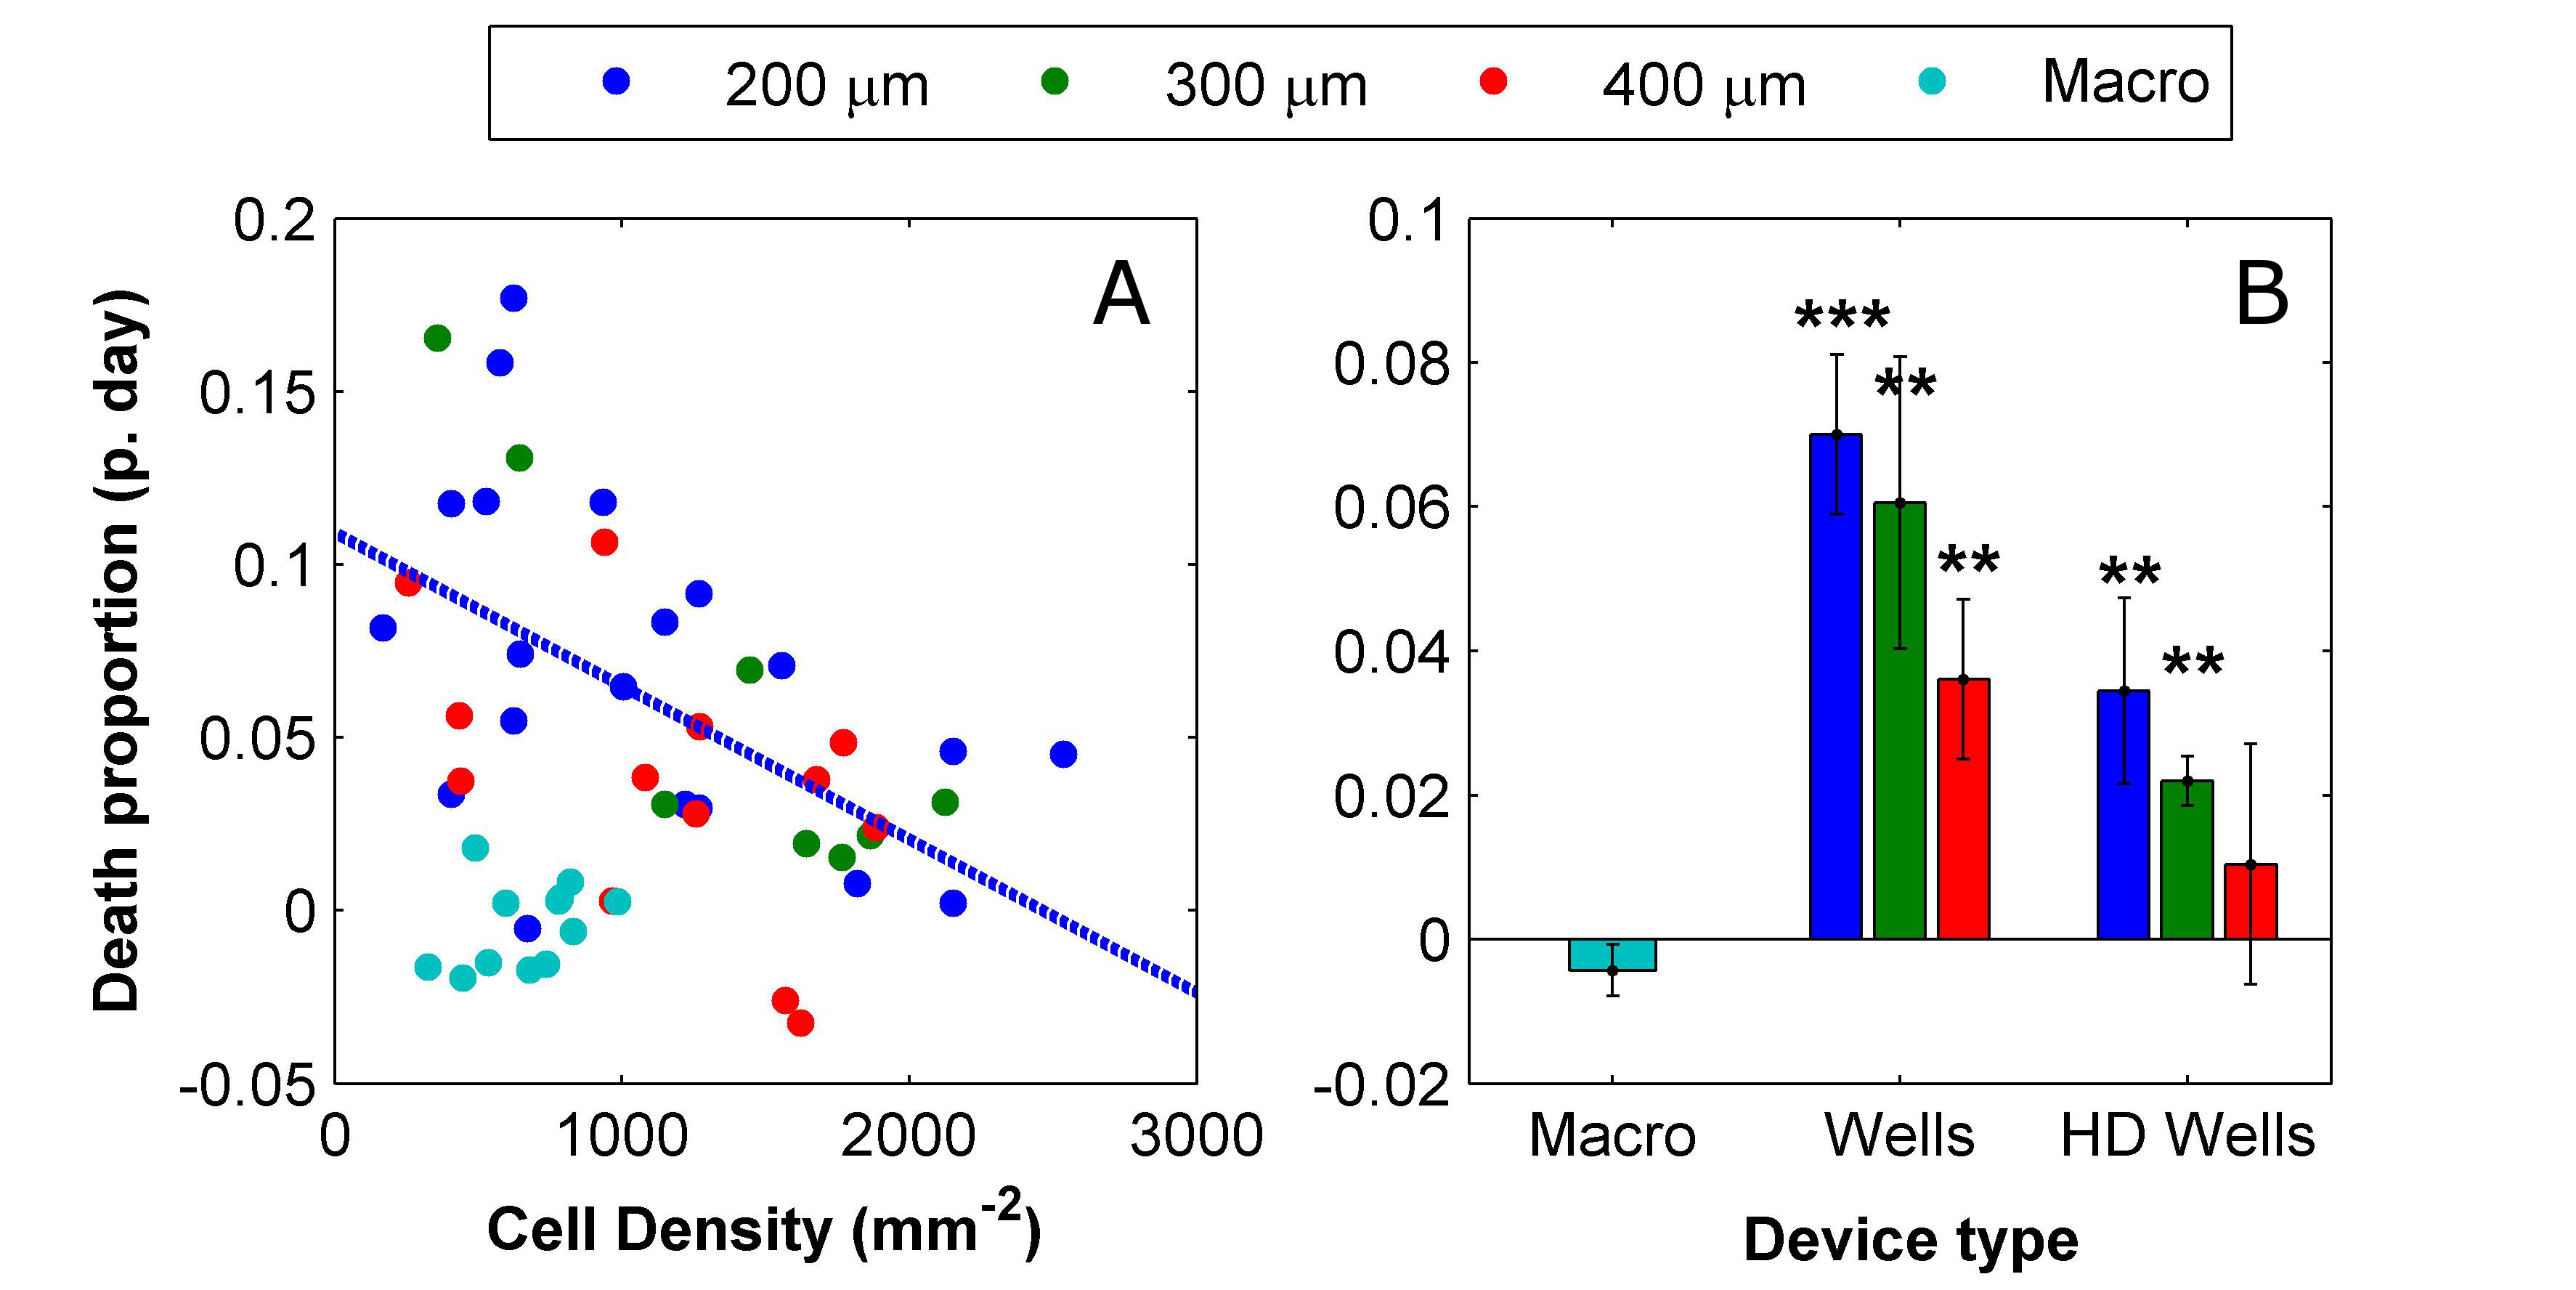
\includegraphics[width=15cm]{chapter4/figures/microWellsStats/mwStats.jpg}
            \caption[Statistics of microculture viability over development]{\textbf{The viability of the microcultures is correlated with their density and size.} (A) Scatter plot of the proportion of dead cells observed in the microcultures and macrocultures between consecutive counting time points as a function of microculture density. Each point represents a comparison between counts at 2 consecutive time points. Cells were counted at 1, 5 and 12 days \textit{in vitro}. Death proportion is normalized to the number of days between the counts. Data is color coded according to microwell size or if it is a macroculture. (B) Comparison of mean proportional death rates between all the microcultures or microcultures with density higher than \(1500 cells\cdot mm^{-2}\) and macrocultures. The data is based on 44 microcultures and 9 macrocultures from 4 different platings.}
            \label{fig:devices:mwStats}
        \end{figure}

        We would like to conclude this section by making a note about the quality of isolation of the microcultures. Since the devices considered here were assembled using plasma bonding, the surface treatment had to follow the `bind-then-surface' approach. This means that the assembled devices were filled and incubated with surface coating solution (PLL) so all exposed internal surfaces were actually chemically prepared for cell adhesion. This means that cells from within the wells were free to send neurites out onto the PDMS surface and even to migrate there. Additionally, the flushing procedure applied after the seeding was imperfect and sometimes left a substantial amount of cells on the PDMS sheet surface. This lack of restriction meant that after two weeks of growth the microcultures had significant innervation from neurons outside of the well (figure \ref{fig:devices:mwIso}). Axons seemed to traverse the entire distance between the the microwells and the large support well which was located \(3.7 mm\) away. This lack of isolation defeats the purpose for which the microwells were designed. This issue is solved in chapter \ref{chap:microculturePulses} where tape based design allows a `surface-then-bond' approach whereby only the well bottom is chemically prepared for cell adhesion.


        \begin{figure}[h]
            \centering
            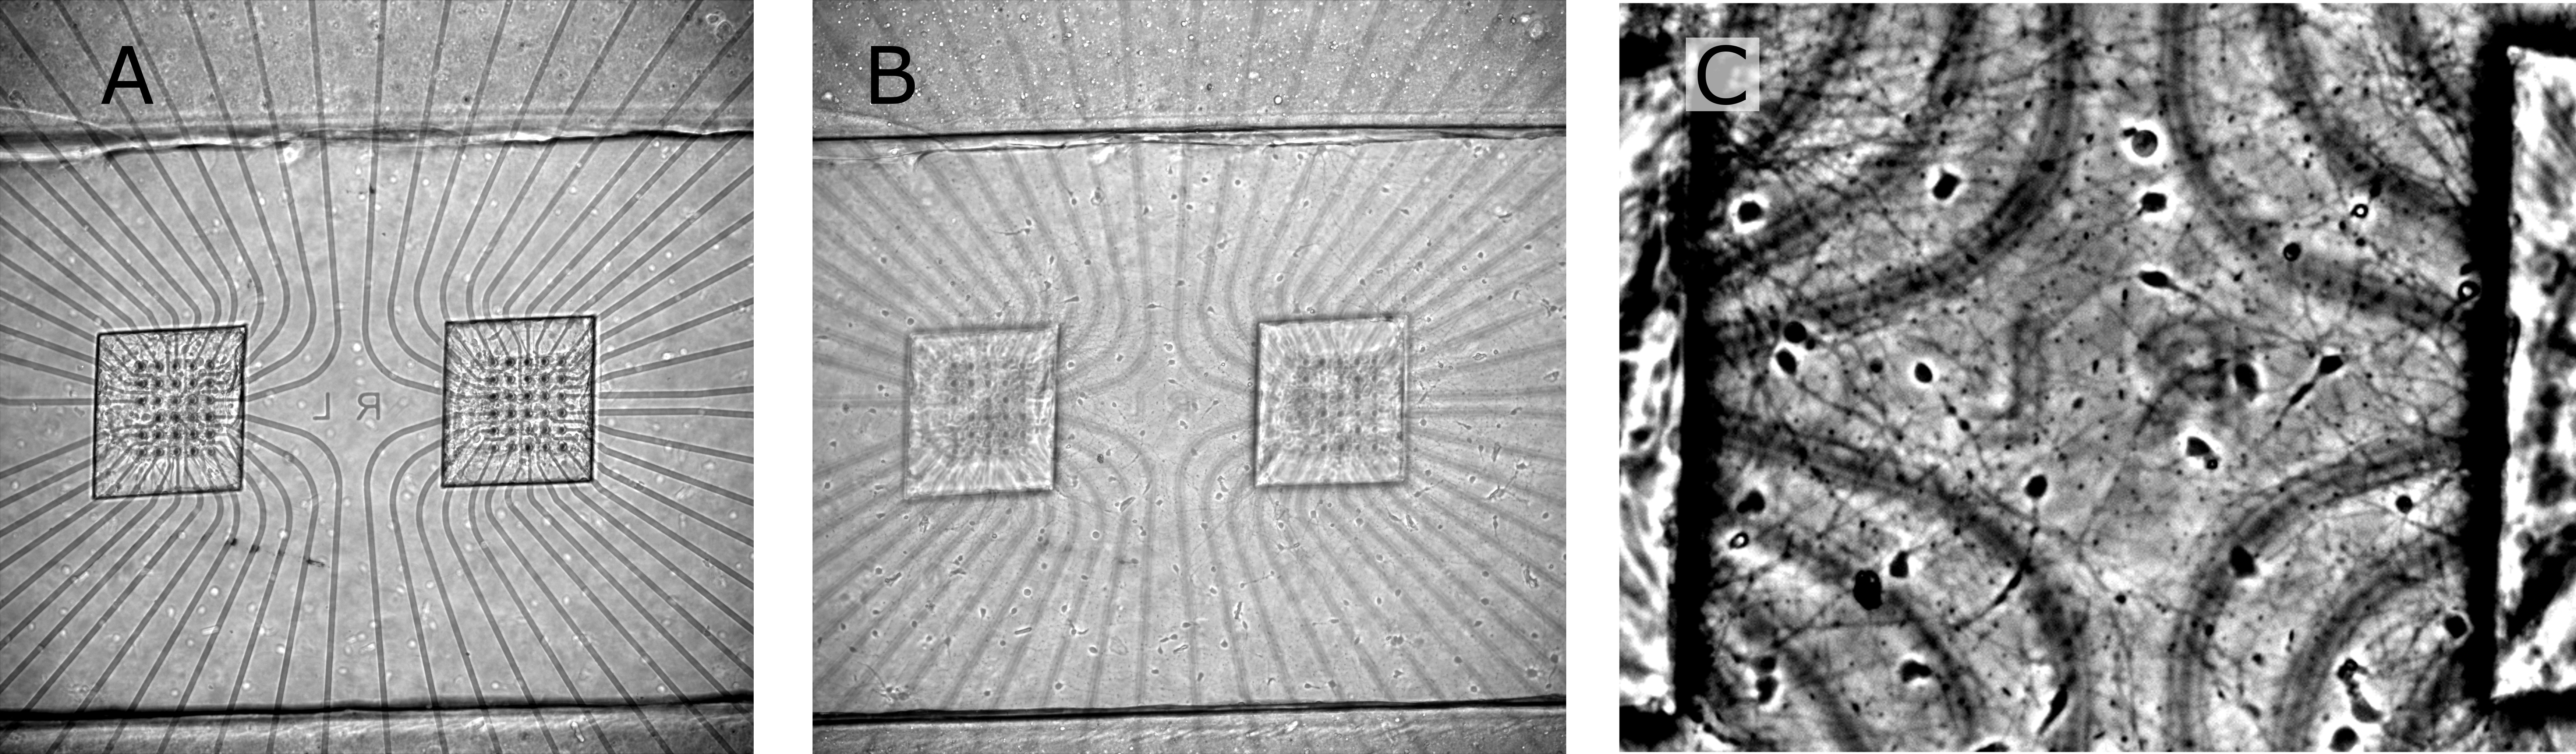
\includegraphics[width=15cm]{chapter4/figures/microWellsIsolation/isolationIssue.jpg}
            \caption[Demonstration of the microculture isolation issue with the bond-then-surface approach]{\textbf{Microcultures are not well restricted to the microwell area with bond-then-surface approach.} (A) Image of microcultures growing on top of commercial microelectrode arrays at 12 days \textit{in vitro}. (B) Image of the same view field as in A focused on the top surface of the PDMS sheet. This image reveals the substantial inhabitation of the top surface by cells and neurites. (C) A zoom into the area between the microwells in B to highlight the presence of neurons and neurites outside the microwells. Microwells are of sizes \(300\times270 \mu m^2 (L\times W)\) for scale reference.}
            \label{fig:devices:mwIso}
        \end{figure}



\section{Viability of neuronal cultures under steady microfluidic flow}
\label{sec:devices:viability}

\subsection{Pilot flow study}
    The operation of the agonist delivery system involves subjecting the neurons to flow rates in the order of millimeter per second. Thus, in this section as well as in chapter \ref{chap:activityAndFlow}, we address the question of how well the cultures perform under flow. Primary neurons are considered to be highly sensitive to shear stresses so we suspected that subjecting them to flow might be deleterious and that there might be a limit to how high a flow rate they can bare. Since the interaction of primary neurons with flow is under investigated we conducted preliminary experiments where cultures at various ages were subjected to steady flow with growth media while being continuously monitored via time lapse imaging. The flow apparatus used for these experiments is described in section \ref{sec:methods:flow}. These experiments seemed to develop in a stereotypical pattern: shortly after initiation of flow, the cells started losing the surface adhesion which was manifested by obvious fasciculation. In younger cultures where not too much ECM had been built it could be observed that the fasciculation was accompanied by a retraction of processes (figure \ref{fig:devices:degeneration}). By 20 hours, most of the cells appeared to degenerate. In older cultures rich in ECM this degeneration also involved complete detachment of the tissue, which was left floating inside the device volume (figure \ref{fig:app:culturePeel}).

    \begin{figure}[!htb]
            \centering
            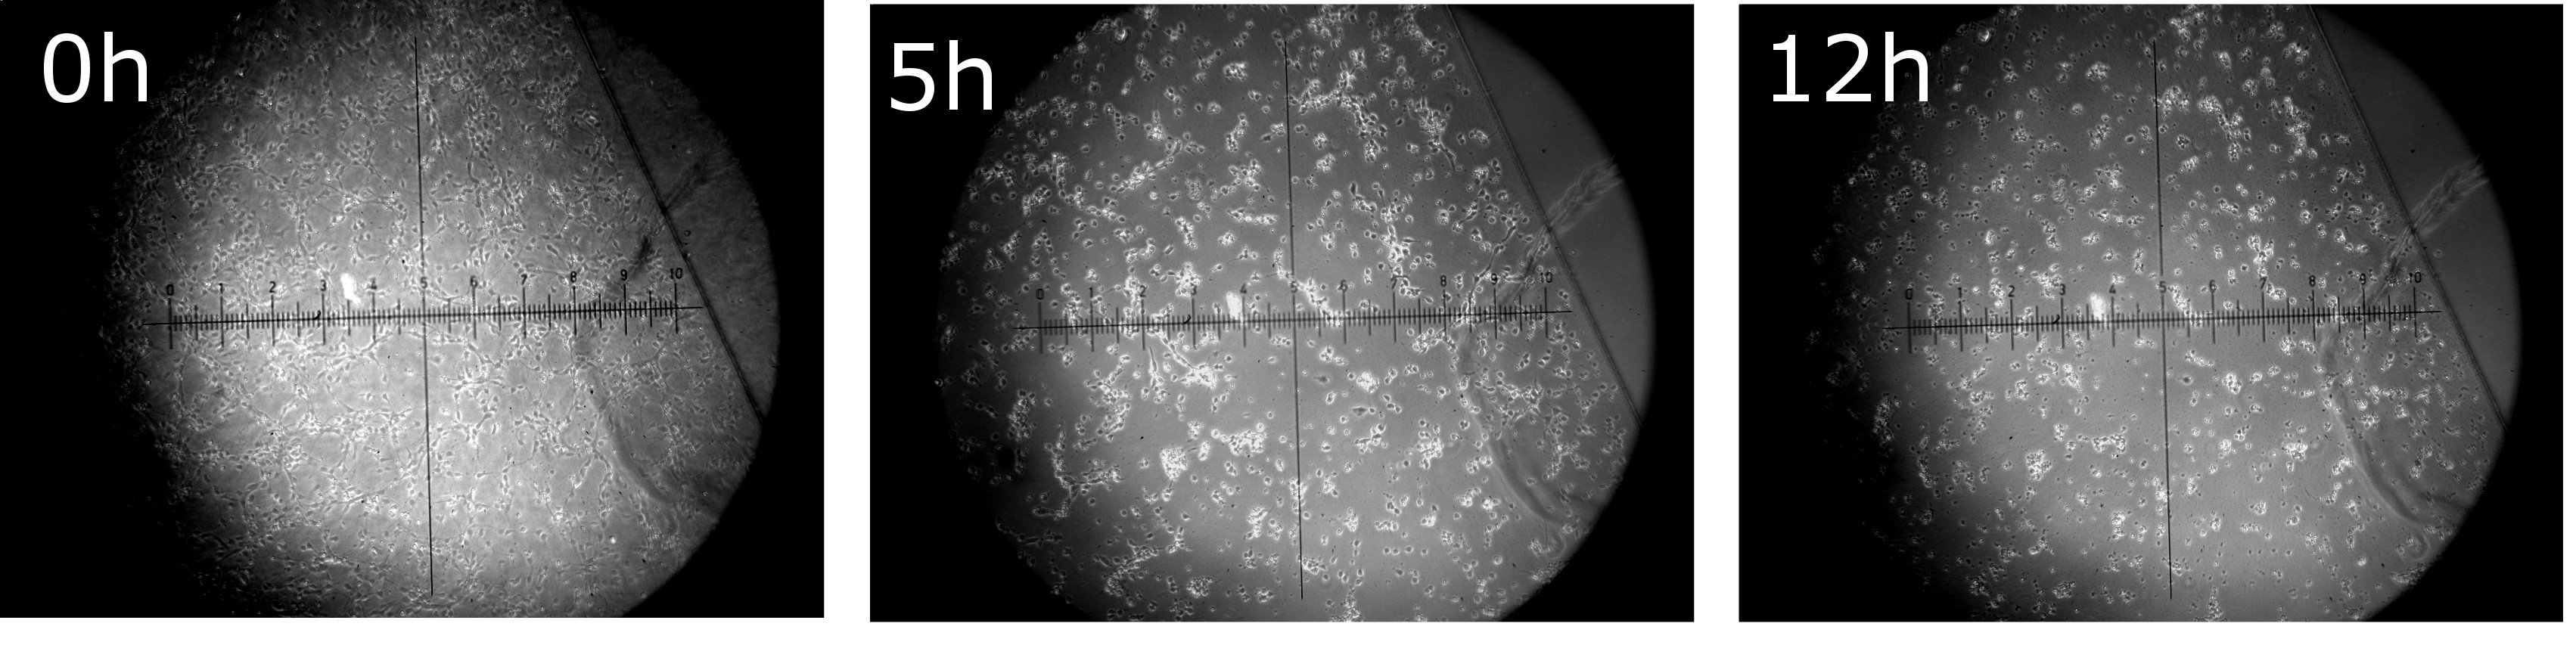
\includegraphics[width=7cm]{chapter4/figures/degenerationExample/degenerationExample.jpg}
            \caption[Time lapse of neuronal culture under steady microfluidic flow]{\textbf{Neuronal cultures exposed to steady flow lose their surface adhesion, retract their processes and degenerate after several hours.} Time lapse of a neuronal culture grown in the standard 1-layer microfluidic devices (section \ref{sec:devices:protocolDev}) placed under flow at 1 day \textit{in vitro}. The flow rate was \(1 nl\cdot s^{-1}\). Scale units: \(\approx100 \mu m\).}
            \label{fig:devices:degeneration}
    \end{figure}

    Initial experiments were conducted with the devices placed openly in the ambient environment while only plugged into a custom made heater system where heating resistors were brought into contact with the glass and the PDMS bulk and were controlled to \(37\degree C\) \cite{johnstoneThesis}. However, we had concerns as to how well this system controls the internal device temperature given that media at room temperature is pumped in. Additionally, maintenance of media CO\textsubscript{2} levels was based on connecting the pressure control system to a 5\% CO\textsubscript{2} / 95\% air gas supply. This configuration assured that the media in the flow reservoirs were fully CO\textsubscript{2} saturated but there was still a concern that as it travels through the tubes in the ambient air some CO\textsubscript{2} content could escape. To alleviate these issue, we built a custom made compact environmental chamber whose internal environment was controlled to \(37\degree C\) and 5\% CO\textsubscript{2} (figure \ref{fig:app:chamber}). The flow tubes were introduced into the environmental chamber through a small side hole before connecting to the devices. The tube configuration was purposefully selected such that the total tubing volume outside the environmental chamber was 3 times less than that of the internal tubing (\(\approx 16 \mu L\) vs. \(\approx 60\mu L\)). This meant that, while travelling from the reservoir to the device, the media spent triple the time inside the chamber environment than in the ambient one so any CO\textsubscript{2} lost outside would necessarily have been reabsorbed. We also calculated that the residence time inside the chamber is at least 10 minutes which is more than enough to heat the media to \(37\degree C\) given the micrometer scale of the tubing (this was verified with an inline flow thermocouple, PH-01, Multi Channel Systems). Nevertheless, the employment of the chamber did little to change the outcome of the flow experiments leading us to conclude that the basic physiological parameters of temperature and media CO\textsubscript{2} saturation did not play a major role in the degeneration.

    Since conditioning factors are known to exert a protective effect on neuronal culture \cite{kaech2006culturing,banker1980trophic} we explored the option of using conditioned media, i.e., media taken from a different culture for flow. We found that this had a pronounced effect on the cultures' tolerance in the sense that there was an initial flow period where the cultures' appearance did not seem to change. Additionally, even though fasciculation and degeneration still occurred, they developed much later, typically more than 10 hours into the flow session. Another interesting observation was that the rapid degeneration observed with fresh media flow seemed to occur regardless of the flow rate and presented itself even when the tubes were connected but the flow was set to \(0 nl\cdot s^{-1}\). These observations suggested that, when using conditioned media, a time window could be present where the culture is functional and useful experiments may be performed. They were also surprising in that the flow rate, i.e., shear, appeared to play a smaller than expected role in the adverse effects of flow. We therefore decided to conduct a systematic study to quantitatively assess the effect of conditioning and shear on the viability under flow and to establish what is the practical experimentation time window.


    \subsection{Quantitative viability analysis}
    \label{sec:devices:viabilityAssay}
    Analyzing how media conditioning affects viability under flow requires an analytic measure of conditioning. Since conditioning involves a continuous secretion of factors into the bulk media, it seemed plausible that, a conditioning scale would be proportional to the length of time which the media was in contact with the cells. We produced conditioned media by growing cortical rat cultures of prescribed densities in T-25 flasks with prescribed media volumes and without changing of the media. The precise protocol and the conditioning scale are provided in section \ref{sec:methods:cond}. Roughly, every 3 days of incubation in the flasks \textit{in vitro} are equivalent to 1 conditioning units.

    \begin{figure}[h]
            \centering
            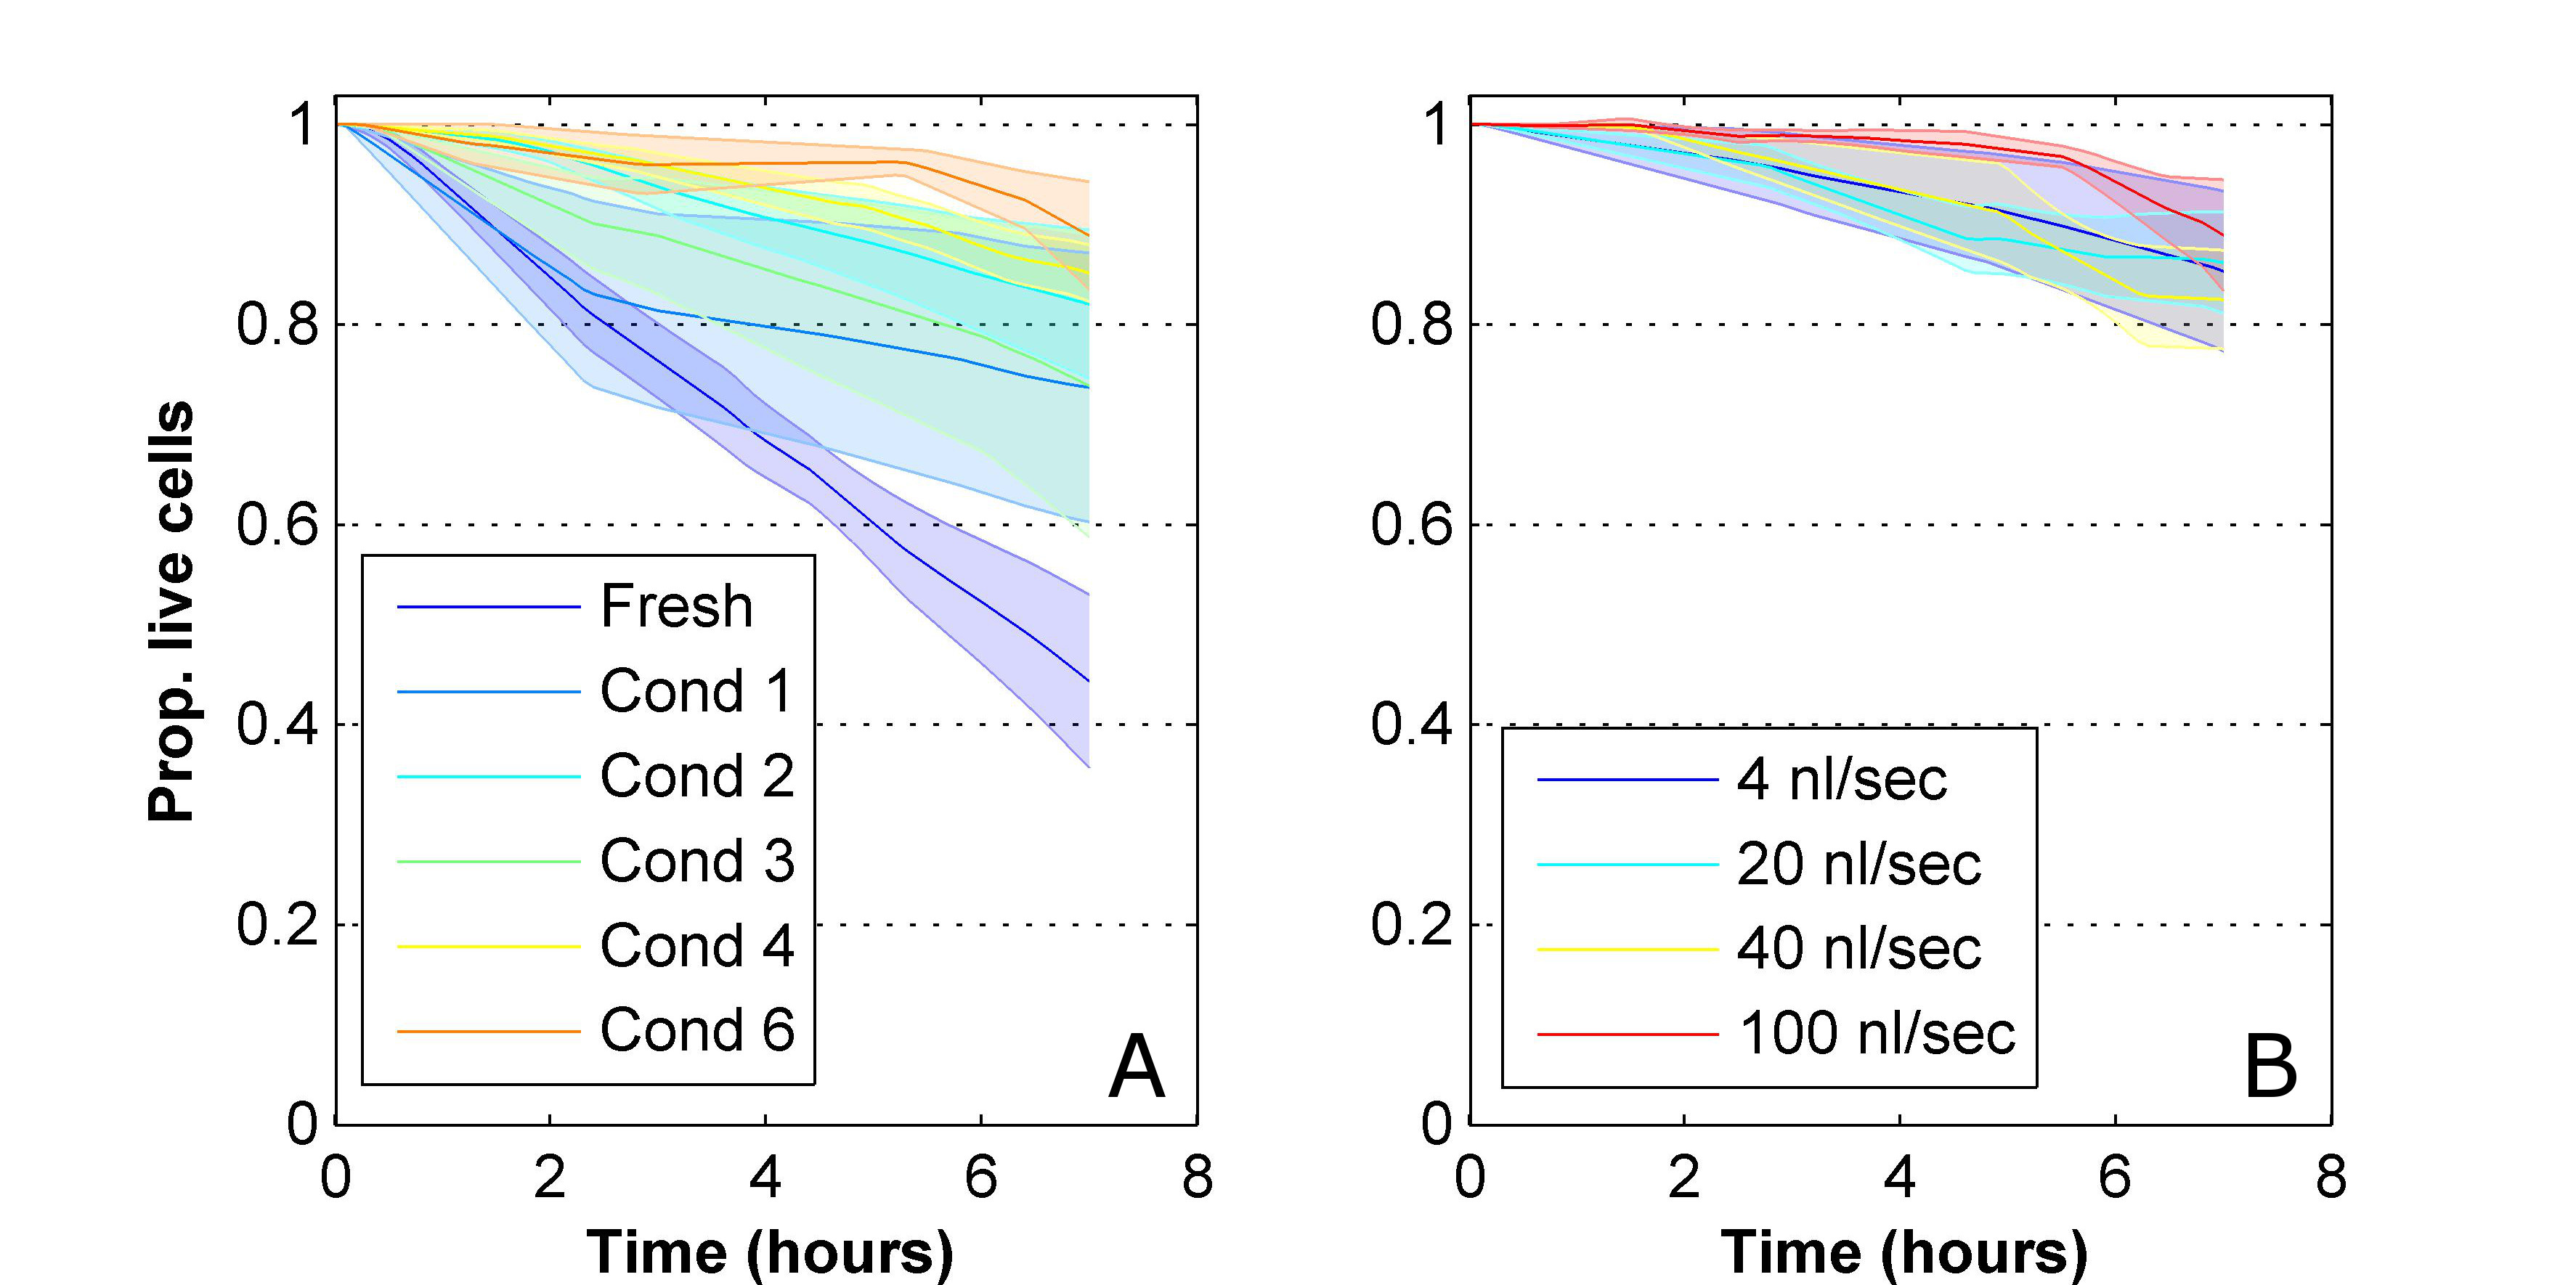
\includegraphics[width=15cm]{chapter4/figures/condImpression/condImpression.jpg}
            \caption[Effect of media conditioning and flow rate on viability of neuronal cultures under steady microfluidic flow]{\textbf{Using conditioned media for flow can significantly prolong the culture viability regardless of the flow rate.} (A) Averaged viability curves for flow with media of increasing conditioning levels. Every curve averages data from several flow experiments where a propidium iodide assay was used to quantitatively assess the number of dead cells over time (full description is given in full in section \ref{sec:methods:flow}). Example for such individual flow curves can be seen in figure \ref{fig:devices:viabilityDetAnalysis}. The flow rate for all experiments was \(40 nl\cdot s^{-1}\). Shaded areas depict the SEM. (B) Averaged viability curves as in A but where the flow rates are varied whereas the conditioning level is fixed at 4. The data is based on 36 experiments from 9 platings. Every curve except for Cond 6 in panel A is the average of at least 3 experiments from 2 different platings. Cond 6 is based on 2 experiments from one plating.}
            \label{fig:devices:viabilityImpression}

    \end{figure}


    We ran a large set of steady flow experiments on macrocultures growing in standard 1-layer devices. The experiments were conducted in a range of conditioning levels and flow rates. To provide a quantitative measure of viability these flow experiments also included a propidium iodide assay (protocol and example in section \ref{sec:methods:flow}). In brief, propidium iodide was added to the flow medium so it was present around the cells for the length of the experiment. Intact plasma membranes of healthy cells are impermeable to this fluorescent DNA-binding molecule. However, when cells die their nuclear material becomes accessible and readily serve as a seed for propidium aggregation and therefore appears as a dot in fluorescent microscopy. These dots were counted to provide a quantitative measure of how many cells have died since the initiation of the flow. During a flow experiment fluorescent images were taken every 1-2 hours to generate a curve of the deterioration in viability. Figure \ref{fig:devices:viabilityImpression} shows averaged viability curves for a range of conditioning levels where the flow rate is fixed and for a range of flow rates where the conditioning level is fixed. The observations made in the previous section are clearly manifested in these curves: increasing of the conditioning levels is negatively correlated with the death rates whereas increase in flow rates within the tested range is not.

    \begin{figure}[!htb]
            \centering
            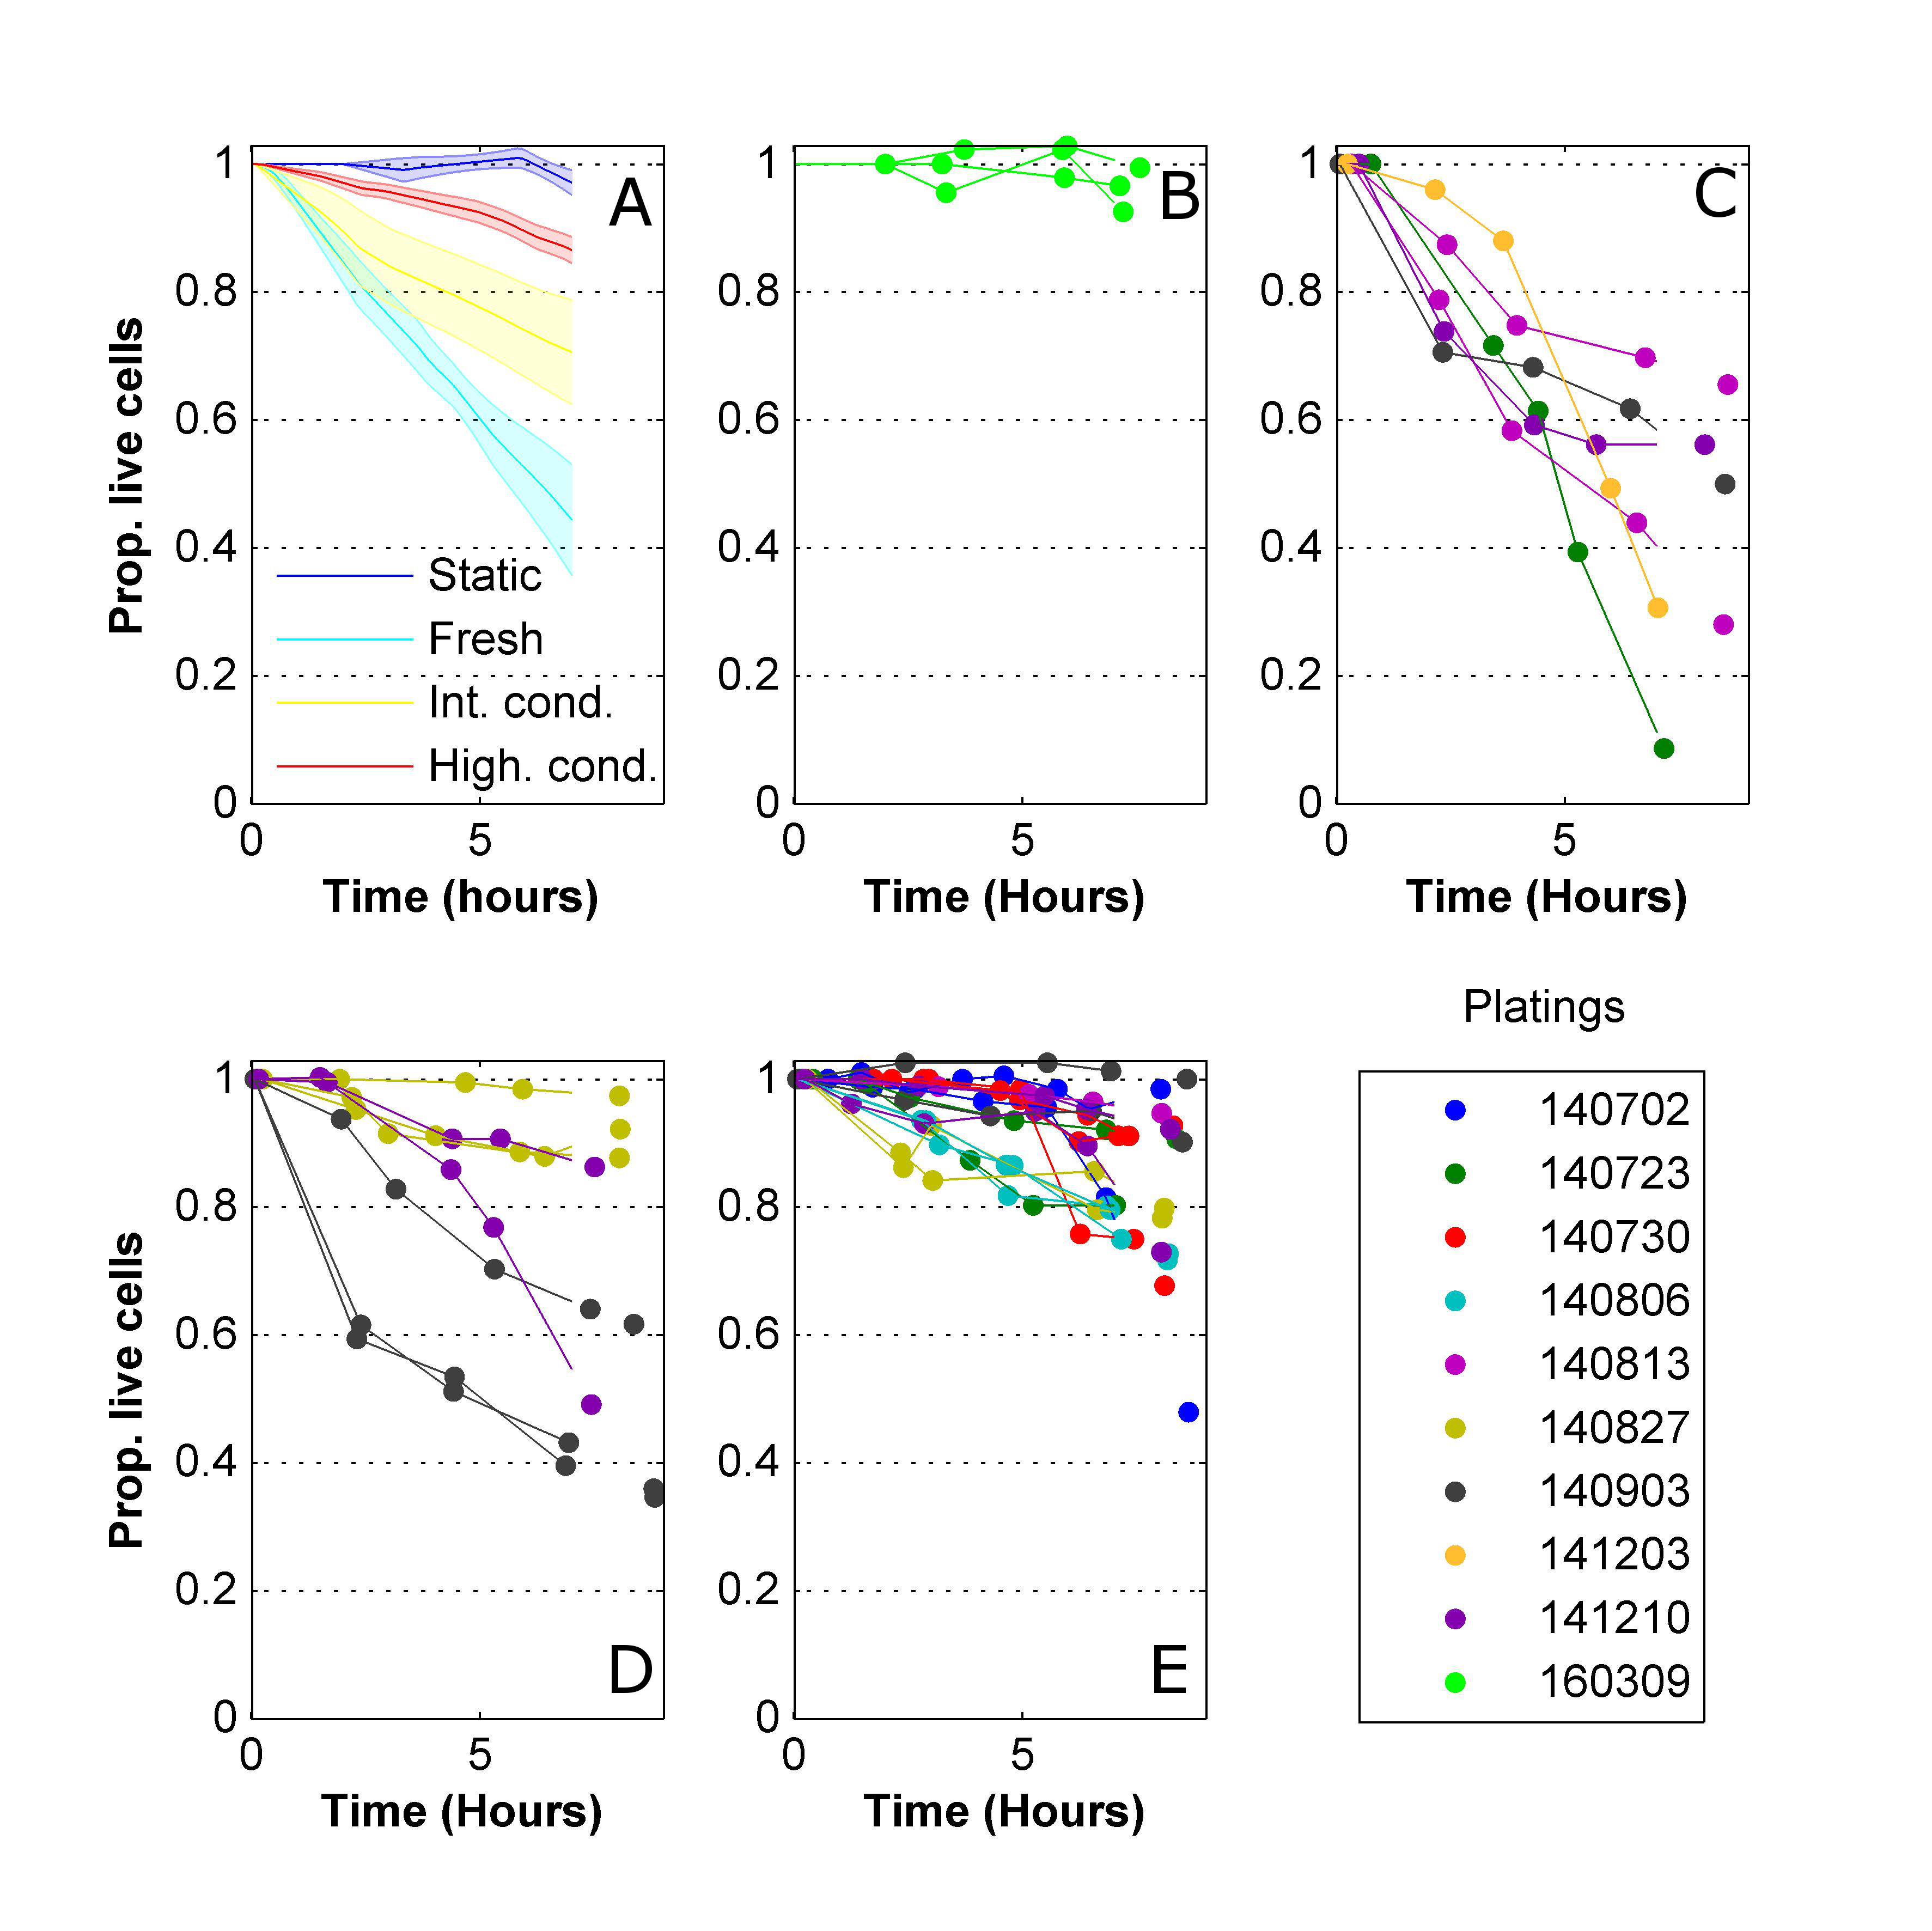
\includegraphics[width=15cm]{chapter4/figures/condDetAnalysis/condDetAnalysis.jpg}
            \caption[Example of viability curves from individual steady flow experiments]{\textbf{Individual viability curves do not exhibit any common temporal features so their average is linear.} (A) Averaged viability curves for increasing conditioning levels as in figure \ref{fig:devices:viabilityImpression} A but with a grouping applied to get improved separation (grouping specified in the text). The flow rate for all experiments was \(40 nl\cdot s^{-1}\). An additional control curve is included where the devices were not connected to the flow system. (B-E) Individual viability curves from the experiments that were averaged in A. Each dot represents a fluorescent image where the number of dead cells were counted. The order of the panels B-E matches the order of the averaged curves as listed in the legend of panel A. Individual curves are color coded according to the date of plating of the given culture.}
            \label{fig:devices:viabilityDetAnalysis}
    \end{figure}



    To facilitate the statistical analysis we grouped the conditioning scale into 3 groups: Fresh media (same as before), intermediately conditioned (grouping conditioning levels 1 and 2) and highly conditioned (grouping levels 3-6). Figure \ref{fig:devices:viabilityDetAnalysis} shows the averaged viability curves generated with new grouping as well as a control curve made without connecting the cultures to the flow system at all (static). The figure also shows a breakdown of the averaged curves into the constituent individual ones per experiment. Since the individual curves did not exhibit any conspicuous common time dependent features and as the averaged curves were strikingly linear we reasoned that a fixed death rate model (linear) would be a plausible a description of this data. In accordance with this notion, the statistical analysis was based on fitting a line to the viability time series of each experiment with a forced intercept at (time=0, viability=1). The statistical testing was then performed on the fitted slopes and is discussed next.

    \begin{figure}[!htb]
            \centering
            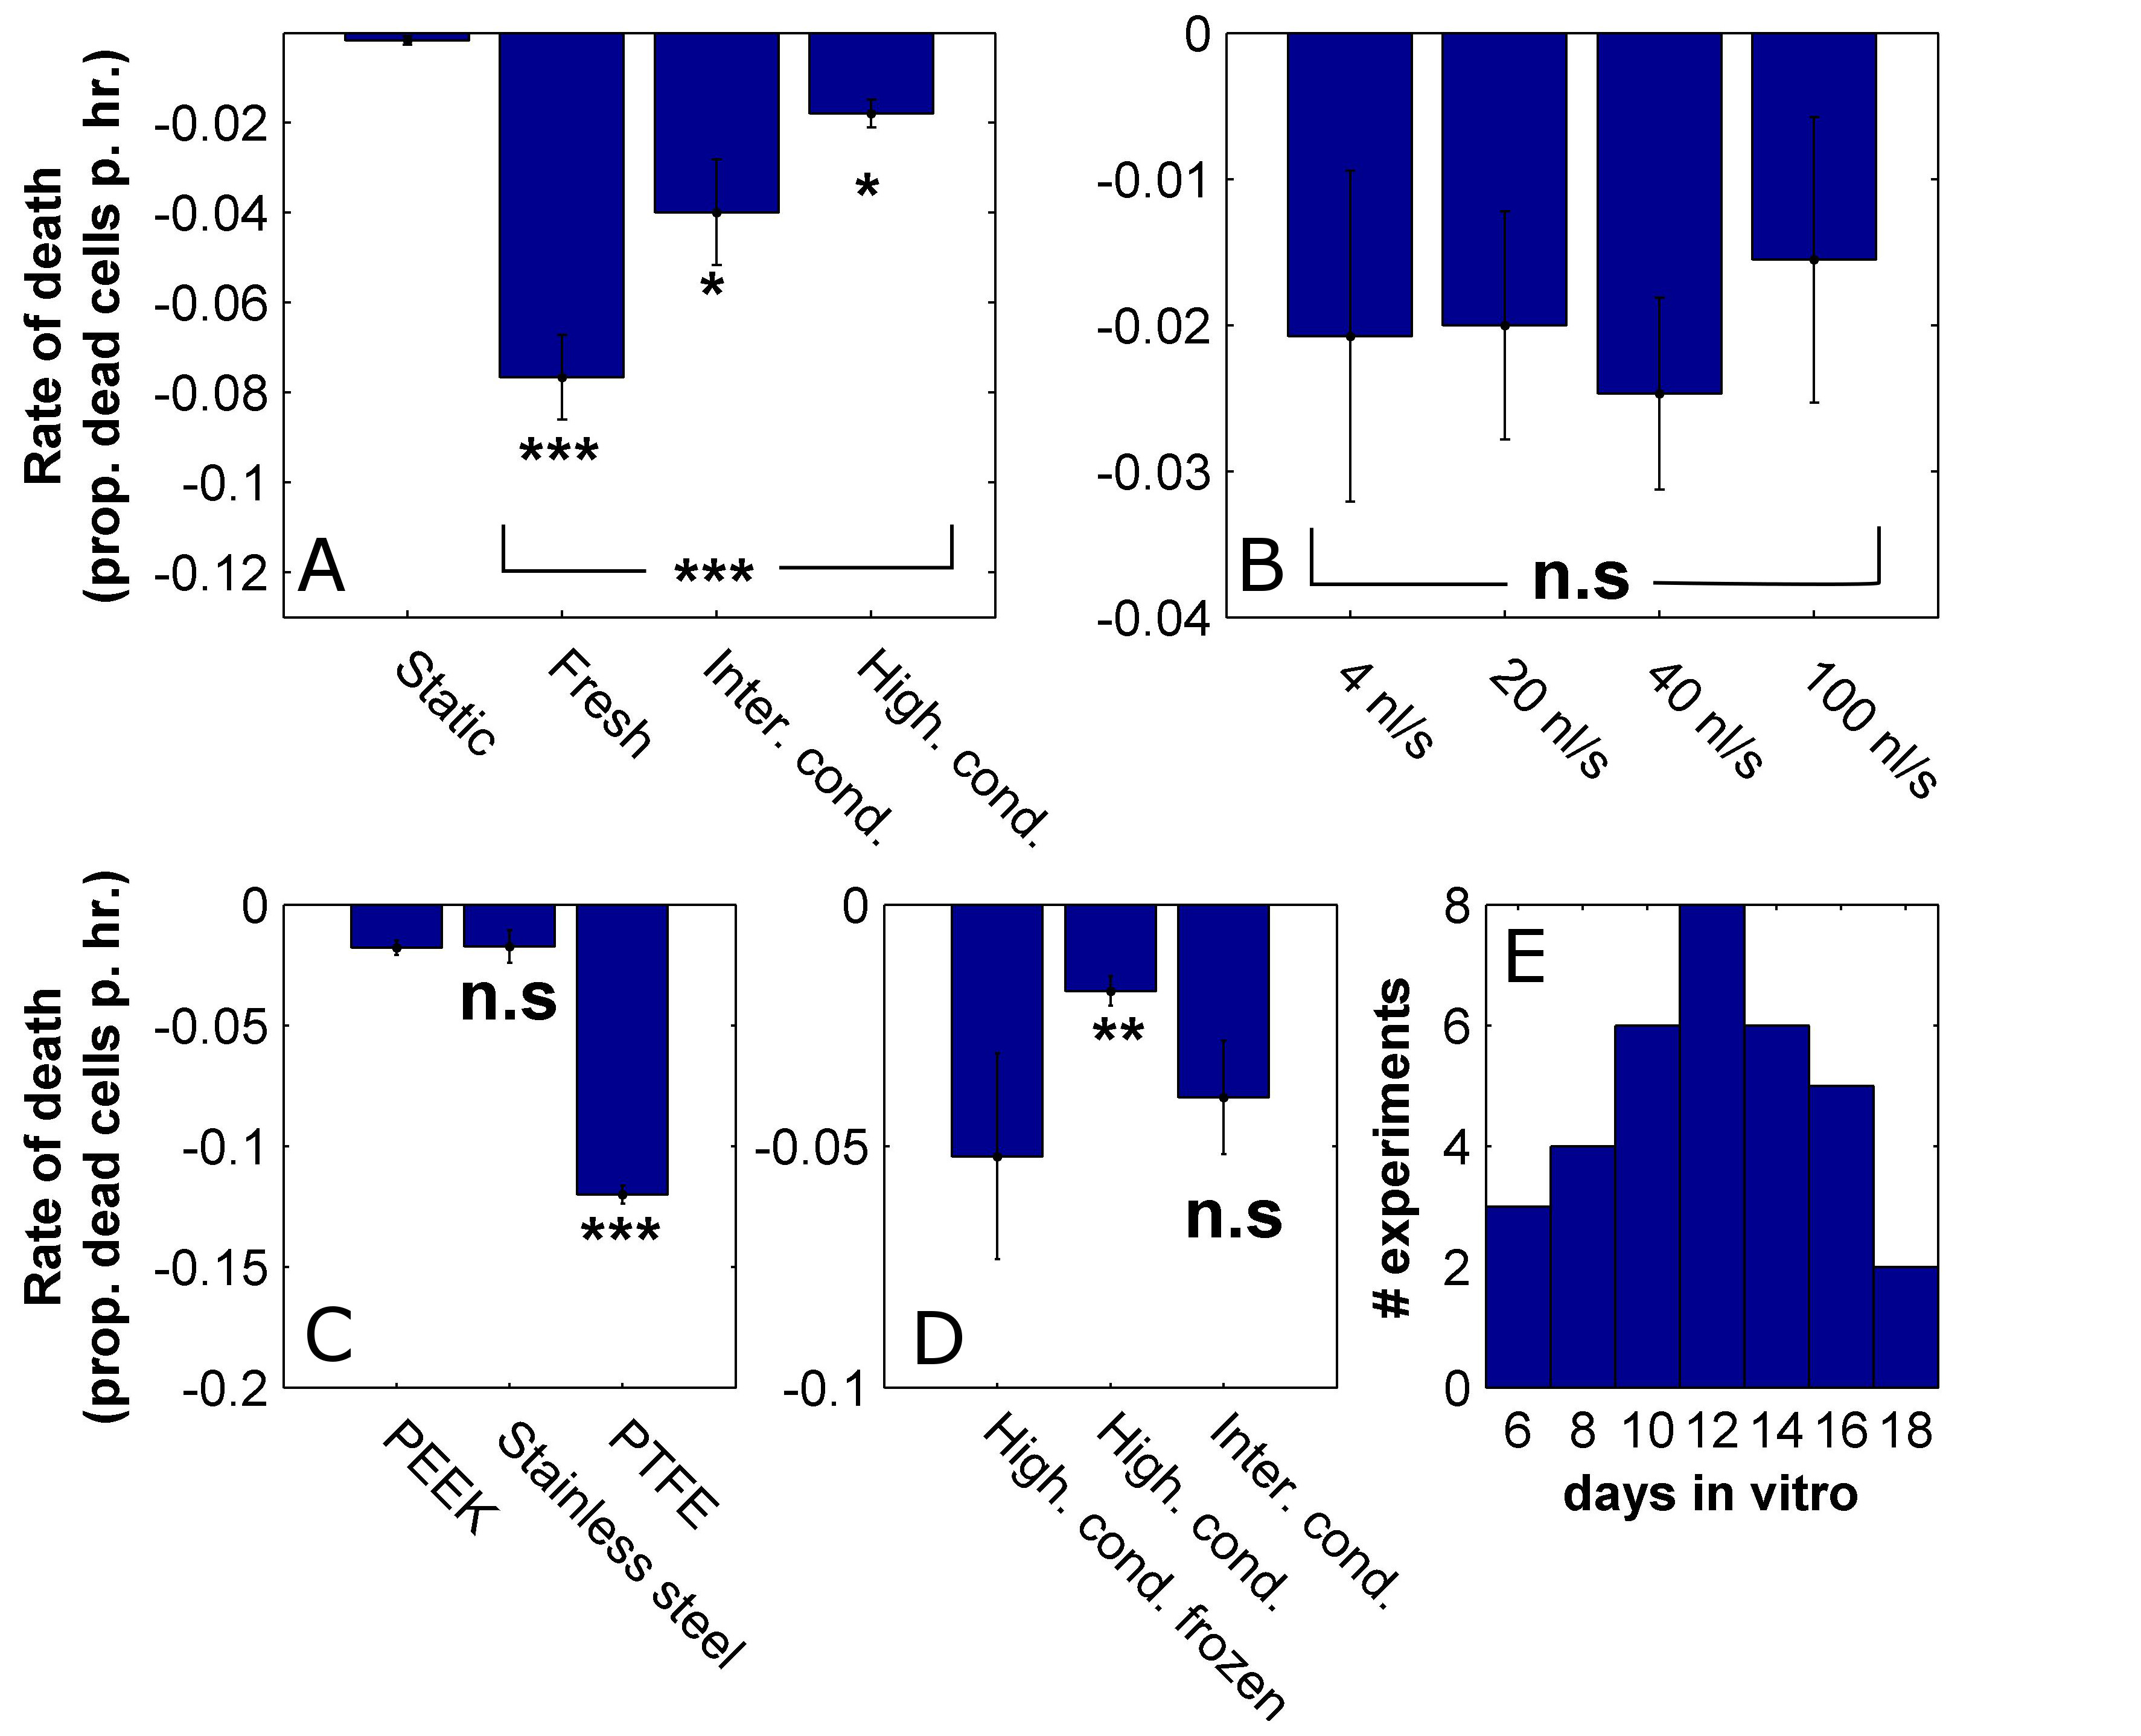
\includegraphics[width=15cm]{chapter4/figures/viabilityStats/viabilityStats.jpg}
            \caption[Statistics of death rates for various steady flow conditions]{\textbf{Death rates under steady flow depend on media conditioning levels and on the type of flow tubes but not on flow rates in the tested range.} (A) Comparison between the measured death rates under steady flow for increasing media conditioning levels and for control devices. Experiments were identical in all other parameters (flow rate \(40 nl\cdot s^{-1}\) and PEEK tubing). (B) Comparison between the measured death rates under steady flow for increasing flow rates (all highly conditioned media, PEEK) (C)  Comparison between the measured death rates under steady flow for different tube types (all highly conditioned media, \(40 nl\cdot s^{-1}\)). (D) Comparison between the measured death rates for conditioned media that was frozen and re-thawed and conditioned media that was directly used (\(40 nl\cdot s^{-1}\), PEEK). (E) Distribution of the ages of the cultures used in this study. The data is based on 49 experiments from 9 platings. Every bar is based on data from at least 3 experiments from 2 different platings except for the static data in panel A and the PTFE data in panel C which are each based on 3 experiments from one plating. Asterisks that group several bars indicate statistical significance of an ANOVA test. Asterisks next to individual bars indicate statistical significance of a t-test between the leftmost condition and the condition at hand. *, **, ***, n.s indicate statistical significance at a level of confidence of 95\%, 99\%, 99.9\% or \textless95\%, respectively.}
            \label{fig:devices:viabilityStats}

    \end{figure}


    Figure \ref{fig:devices:viabilityStats} shows a comparison of the fitted death rate slopes for various flow conditions. The conditioning levels of the flow media ware shown to have a significant effect on the death rate (Figure \ref{fig:devices:viabilityStats} A, 1-way ANOVA, \(p=1.5\times 10^{-5}\)). However, flow under all conditioning levels still resulted in death rates significantly higher than control (unbalanced t-tests, \(p=2.1\times 10^{-4}\), \(0.049\) and \(0.021\) for fresh media, intermediately conditioned and highly conditioned respectively). Thus were were not able to find a conditioning regime where the cultures were viable for long term under flow. To get an idea as to how much using conditioned media can extend the experimentation time, we calculated how long at least 90\% of the cells will be alive, given the established death rates. This provided times of 1.3, 2.5 and 5.6 hours respectively for the 3 conditioning levels at hand. Given that highly conditioned media was used, changing the flow rate did not produce a significant difference (Figure \ref{fig:devices:viabilityStats} B, 1-way ANOVA, \(p=0.91\)). The main experiments above were performed with PEEK tubing (see section \ref{sec:methods:flow}). We also tested if changing the tubing material would affect the viability under flow. We found that stainless steel tubing gave the same results as the PEEK for flow with highly conditioned media. PTFE tubing, however, was surprisingly associated with a significantly higher rate of degeneration (Figure \ref{fig:devices:viabilityStats} C, unbalanced t-tests, \(p=0.95\) and \(7.5\times 10^{-11}\) for stainless steel and PTFE tubing, respectively). Thus, the beneficial effect of conditioning seems to be absent when using PTFE. This could suggest that our PTFE tubing absorbs valuable conditioning factors or that it introduces contaminants into the media during flow. We did not further interrogate this non-trivial effect but it is important to make a note of how the tubing selection can affect these types of experiments. Finally, since all the conditioned media in this study was used straight from the culture flask we wanted to check whether it could be stored for later use as that would greatly simplify the experimental design. Consequentially, we extracted highly conditioned media, kept it frozen at \(-80\degree C\) for several weeks and then heated it back up to \(37\degree C\) prior to using it for flow. We found that the frozen media did not preserve the beneficial effects of the conditioning and resulted in significantly faster death rates as compared to the media used directly from the flasks (\ref{fig:devices:viabilityStats} D, unbalanced t-test, \(p=0.0073\)). Interestingly, the performance of the frozen media was statistically the same as that of the intermediately conditioned media (unbalanced t-test, \(p=0.59\)) so the benefits of conditioning were still partially present. It is likely that some of the conditioning factors degrade over time and are sensitive to freezing and thawing (e.g., large protein molecules) hence the above results.


\section{Chapter conclusion}
     \label{sec:devices:conclusion}
     In this chapter, we demonstrated a capacity for growing rat macrocultures (standard size) and microcultures in microfluidic devices. The observations made in sections \ref{sec:devices:circulation} and \ref{sec:devices:microcultures} highlight the challenges that exists in the design of microfluidic devices for neuronal culture in finding a `goldilocks' circulation regime. On one hand, enough nutrients and oxygen need to be allowed into the device to meet the requirements of the culture and, on the other hand, conditioning factors must be prevented from `escaping' as they are required for sustaining the development. The precise design is strongly dependent on the size and density of the culture as these inform its oxygen and nutrient requirements and also the secretion rate of conditioning factors.

     In the second part of this chapter we used a viability assay to quantitatively observe the cultures' health under flow. We found that using highly conditioned media can sustain the viability of the culture for several hours under flow and therefore consider it a promising approach for establishment of the system. Interestingly, the shear rate induced by the flow did not correlate with the viability which suggests that the deleterious effects are mediated solely by removal of conditioning factors and not at all by physical shear. Nevertheless, this is not the only possible interpretation for these results. A related study testing the viability of neuronal culture under a range of flow rates reported a shear threshold associated with culture degeneration \cite{liu2013galanin}. This study found that a compound isolated from brain tissue named Galanin protects the cultures from the shear so that, when it is introduced into the flow media, an effective increase in the degeneration threshold is observed. A possible interpretation of our results could therefore be that the conditioned media contains factors similar to Galanin that protect the cells from the shear and therefore effectively increase the flow rate threshold to a level exceeding the tested range. The study presented here cannot unambiguously distinguish the above-described narratives. This issue will be further addressed in the next chapter where electrophysiological measurements under flow will be presented and shed light on the mechanisms by which flow interacts with the culture.



